\documentclass[9pt]{beamer}
\usepackage[T1]{fontenc}
\usepackage[utf8]{inputenc}
\usepackage{lmodern}
\usepackage[english]{babel}

\usepackage{stmaryrd}
\usepackage{verbatim}
\usepackage{geometry}
\usepackage{setspace}

\usepackage{latex/agda}
\usepackage{unicode-math}
\setmathfont{XITS Math}

\setmainfont{DejaVu Serif}
\setsansfont{DejaVu Sans}
\setmonofont{DejaVu Sans Mono}


\usepackage{newunicodechar}
\newunicodechar{→}{\ensuremath{\mathnormal\to}}
\newunicodechar{ℕ}{\ensuremath{\mathbb{N}}}


\usepackage{xcolor}
\usepackage[normalem]{ulem}
\usepackage{soul}
\usepackage{amsmath}
\usepackage{amssymb}

\usepackage{multirow}
\usepackage{multicol}
\usepackage{caption}
\usepackage{bussproofs}

\usepackage{tikz-cd}
\usetikzlibrary{matrix}

\let\oldquote\quote
\let\endoldquote\endquote

\RenewDocumentEnvironment{quote}{om}
  {\oldquote}
  {\par\nobreak\smallskip
   \hfill(#2\IfValueT{#1}{~---~#1})\endoldquote
   \addvspace{\bigskipamount}}

\newcommand{\equalH}[2]{#1 = #2}
\newcommand{\comprehensionH}[3]{\{ #1 : #2 \mid #3 \}}
\newcommand{\arrowH}[2]{#1 \rightarrow #2}
\newcommand{\appH}[2]{#1 #2}
\newcommand{\equivalenceH}[2]{#1 \simeq #2}

% hott stuff here
\newtheorem{definition}%{Definition}
\newtheorem{lem}{Lemma}
\newtheorem{proof}%{Proof}
\newtheorem{thm}{Theorem}

\newcommand{\jdeq}{\equiv}      % An equality judgment
\newcommand{\refl}[1]{\ensuremath{\mathsf{refl}_{#1}}\xspace}
\newcommand{\define}[1]{\textbf{#1}}
\newcommand{\defeq}{\vcentcolon\equiv}  % A judgmental equality currently being defined

%\newcommand{\jdeq}{\equiv}      % An equality judgment
%\let\judgeq\jdeq


\newcommand{\ind}[1]{\mathsf{ind}_{#1}}
\newcommand{\indid}[1]{\ind{=_{#1}}} % (Martin-Lof) path induction principle for identity types

\newcommand{\blank}{\mathord{\hspace{1pt}\text{--}\hspace{1pt}}}

\newcommand{\opp}[1]{\mathord{{#1}^{-1}}}
\let\rev\opp

\newcommand{\id}[3][]{\ensuremath{#2 =_{#1} #3}\xspace}



\newcommand{\UU}{\ensuremath{\mathcal{U}}\xspace}
\let\bbU\UU
\let\type\UU

\newcommand{\equalH}[2]{#1 = #2}
\newcommand{\comprehensionH}[3]{\{ #1 : #2 \mid #3 \}}
\newcommand{\arrowH}[2]{#1 \rightarrow #2}
\newcommand{\appH}[2]{#1 #2}
\newcommand{\equivalenceH}[2]{#1 \simeq #2}



\usetheme{Antibes}
\usecolortheme{beaver}
\useinnertheme{rounded}
\useoutertheme{infolines}

%\titlegraphic{\includegraphics[width=25mm]{gottingen1.png}}
\title{Modeling Formal Languages in Grammatical Framework}
\subtitle{On the Grammar of Proof}
\author{Warrick Macmillan}
\date{$7^{th}$ August 2021}


\begin{document}

\begin{frame}
  \titlepage
\end{frame}



\section{Overview}

\subsection{Introduction}

\begin{frame}
\frametitle{One Remark}

\begin{alertblock}{~}
I want feedback on this talk, please
\end{alertblock}

\end{frame}

\begin{frame}
\frametitle{Table of Contents}

\begin{enumerate}

\item Explore abstract relationships between mathematics, CS (TT in
  particular), and linguistics
\item Practical and brief intro to MLTT and Agda
\item Grammars elaborating the abstractions above
\item Thoughts about the future and conclusions
\end{enumerate}
\end{frame}

\begin{frame}
\frametitle{Abbreviations}
\begin{itemize}
\item \textbf{TT} : Type Theory
\item \textbf{MLTT} : Martin-Löf Type Theory
\item \textbf{MLTT} : Homotopy Type Theory
\item \textbf{CTT} : Cubical Type Theory
\item \textbf{NL} : Natural Language
\item \textbf{PL} : Programming Language
\item \textbf{GF} : Grammatical Framework
\item \textbf{PGF} : Portable Grammar Format
\item \textbf{ITP} : Interactive Theorem Prover
\item \textbf{FOL} : First Order Logic
\item \textbf{BNF} : Backus-Naur form
\item \textbf{CADE} : Conference on Automated Deduction
\item \textbf{HOL} : Higher Order Logic
\item \textbf{HIT} : Higher Inductive Type
\item \textbf{GADT} : Generalized Algebraic Data Type
\item \textbf{RGL} : Resource Grammar Library
\end{itemize}
\end{frame}

\begin{frame}[fragile]
\frametitle{Abstraction Ladders}
\begin{columns}
\begin{column}{.5\linewidth}
\begin{tikzcd}
Strings \ar[d,"Lexical\ Analysis"] \ar[dd,bend right=+90.0, swap,"Front\ End"]
&[5m]
\\ Lexemes \ar[d,"Parsing"] &[5em]
\\ ASTs \ar[d,"Type\ Checker"] &[5m]
\\ Typed\ ASTs
  \ar[dd, bend left, "Code\ Generator"]
  \ar[dd, bend right, swap, "Interpreter"] &[5m]
\\ ...
\\ Target\ Language
\end{tikzcd}
\end{column}
\begin{column}{0.6 \linewidth}
\begin{tikzcd}
  Phonemes \arrow[d, "Morhphophonological
  \\ Anaylsis" description]
  \\ Morphemes \arrow[d, "Parse"]
  \\ \{\ Syntactic\ Representation\ \} \arrow[d, "Montague"', bend right=49]
    \arrow[d, "Ranta", bend left=49] \arrow[d, "..." description]
  \\ {\{\ STLC,\ ...\ ,\ DTT\ \}} \arrow[d, "?" description]
  \\ {\{\ Nearal Encoding\ ,\ ...\ ,\ I\ Language\ \}} \arrow[d, "?" description]
  \\ Phonemes
\end{tikzcd}
\end{column}
\end{columns}
\end{frame}

\begin{frame}[fragile]
\frametitle{Computational Trinitarianism}
\centering
\begin{tikzcd}
                                                                            &  &  & Logic \arrow[llldddd, "Denotational\ Semantics" description] \arrow[rrrdddd, "Include\ Terms" description] &  &  &                                                                                                       \\
                                                                            &  &  &                                                                                                            &  &  &                                                                                                       \\
                                                                            &  &  &                                                                                                            &  &  &                                                                                                       \\
                                                                            &  &  &                                                                                                            &  &  &                                                                                                       \\
Math \arrow[rrruuuu, "Embedded\ in\ FOL", bend left] \arrow[rrrrrr, "ITP"'] &  &  &                                                                                                            &  &  & CS \arrow[llllll, "Denotational\ Semantics", bend left] \arrow[llluuuu, "Remove\ Terms"', bend right]
\end{tikzcd}


\end{frame}


\begin{frame}[fragile]
% \frametitle{Linguistic  Interpretations}
\frametitle{Interpretation of Language}
\begin{alertblock}{Observation}
  Only semantic interpretations in these domains.
  One may decide on syntactic, pragmatic, or other paradigms to view this through.
\end{alertblock}
\centering
\begin{tikzcd}
     &  &  & Logic                                                                                                                     &  &  &            \\
     &  &  &                                                                                                                           &  &  &            \\
     &  &  & Linguistics \arrow[uu, "Montague\ Semantics"'] \arrow[llldd, "Distributional\ Semantics"'] \arrow[rrrdd, "TT\ Semantics"] &  &  &            \\
     &  &  &                                                                                                                           &  &  &            \\
Math &  &  &                                                                                                                           &  &  & CS\ (MLTT)
\end{tikzcd}

\end{frame}


\begin{frame}[fragile]
\frametitle{Trinitarian Linguistics }
\centering
\begin{tikzcd}
                                                &  &  & Logic \arrow[dd, "Embedding"] &  &  &                               \\
                                                &  &  &                               &  &  &                               \\
                                                &  &  & Linguistics                   &  &  &                               \\
                                                &  &  &                               &  &  &                               \\
Math \arrow[rrruu, "Language\ Of\ Mathematics"] &  &  &
&  &  & CS\ (MLTT) \arrow[llluu, "Meaning\ Explanations"]
\end{tikzcd}

\end{frame}

\begin{frame}[fragile]
\centering
\frametitle{Trinitarian Grammars}
% https://tikzcd.yichuanshen.de/#N4Igdg9gJgpgziAXAbVABwnAlgFyxMJZAZgBoAGAXVJADcBDAGwFcYkQAZCAcywGMQAX1LpMufIRTlSAFmp0mrdgFl6OABZCRIDNjwEiANlnyGLNohABhAMoAdOwAIAFMo4AVdwEotovRKIyACZTRQsQAHEAMSF5GChueCJQADMAJwgAWyRpEBwIJDIQRnoAIxhGAAUxfUlimBScEBozJUsAJXowHHoHRy5ePj7nKwBBABEAUR9hVIzsxABGGnzCmhLyqpqAy0YGppaw9k7u3qcACQgcHGGbAFU+1Q0Z7XSspCCVgsQi1vC+ZilfhMTyxQRAA
\begin{tikzcd}
                                              &  &  & Logic \arrow[dd, "Ranta\
                                              Logic\ (CADE\ 11)"] &  &  &                                       \\
                                              &  &  &                                          &  &  &                                       \\
                                              &  &  & GF                                       &  &  &                                       \\
                                              &  &  &                                          &  &  &                                       \\
Math \arrow[rrruu, "Ranta\ (HoTT\ 14)"] &  &  &                                          &  &  & CS\ (MLTT) \arrow[llluu, "cubicalTT"]
\end{tikzcd}

\end{frame}

\begin{frame}[fragile]
\frametitle{Models of  GF}
\centering
\begin{tikzcd}
     &  &  & Logic                                                                                                                                             &  &  &            \\
     &  &  &                                                                                                                                                   &  &  &            \\
     &  &  & GF \arrow[uu, "GF\ Parser\ Specification"'] \arrow[llldd, "Theory\ of\ Operads"']
     \arrow[rrrdd, "Implementation\ of", bend left] \arrow[rrrdd, "Agda\ Embedding", bend right] &  &  &            \\
     &  &  &                                                                                                                                                   &  &  &            \\
Math &  &  &                                                                                                                                                   &  &  & CS\ (MLTT)
\end{tikzcd}

\end{frame}

\begin{frame}[fragile]
\frametitle{Remarks}

\begin{quote}{Robert Harper, OPLSS}
  Concrete syntax is, in some sense, where programming meets psychology.
\end{quote}

\begin{itemize}
\item Trinitarian doctrine is in the ``formal" space
\item Trinitarianism + linguistics is partially informal and very underexplored
\item Introduces many philosophical concerns
\item Perhaps a rereading of Wittgenstein should take place in this context
\end{itemize}
\end{frame}

\section{Preliminaries and Perspectives}

\subsection{MLTT}

\begin{frame}
\frametitle{Predecessors}

\begin{itemize}
  \item Frege : Formal proof, predicate logic 
  \item Russel : Invents TT to resolve his paradox 
  \item Brouwer : Constructivism
  \item Heyting, Kolmogorov, Church, Gödel, Kleene, Bishop, ...
\end{itemize}

\end{frame}

\begin{frame}

\begin{quote}{Per Martin-Löf, Padua Italy, June 1980}

Mathematical logic and the relation between logic and mathematics have been
interpreted in at least three different ways:
\newline

\\
i. mathematical logic as symbolic logic, or logic using mathematical symbolism; \\
ii. mathematical logic as foundations (or philosophy) of mathematics;\\
iii. mathematical logic as logic studied by mathematical methods, as a branch of mathematics.
\newline

\\
We shall here mainly be interested in mathematical logic in the second sense.
What we shall do is also mathematical logic in the first sense, but certainly
not in the third.
\end{quote}
\end{frame}

\begin{frame}
\frametitle{Props vs Types}

\begin{columns}

\begin{column}{0.4 \textwidth}
\begin{block}{First Order Logic}
  \begin{itemize}
    \item $\forall$
    \item $\exists$
    \item $\supset$
    \item $\wedge$
    \item $\lor$
    \item $\neg$
    \item $\top$
    \item $\bot$
    \item $=$
  \end{itemize}
\end{block}
\end{column}

\begin{column}{0.4 \textwidth}
\begin{block}{Dependent Type Theory}
  \begin{itemize}
    \item $\Pi$
    \item $\Sigma$
    \item $\to$
    \item $\times$
    \item $+$
    \item $\neg$
    \item $\top$
    \item $\bot$
    \item $\equiv$
  \end{itemize}
\end{block}
\end{column}

\end{columns}

\end{frame}

\begin{frame}
\frametitle{Sets vs Types}
\begin{columns}

\begin{column}{0.4 \textwidth}
\begin{exampleblock}{Sets}
  \begin{itemize}
    \item $\mathbb{N}$
    \item $\mathbb{N} \times \mathbb{N}$
    \item $\mathbb{N} \to \mathbb{N}$
    \item $\{x|P(x)\}$
    \item $\emptyset$
    \item $?$
    \item $\cup$
    \item $?$
  \end{itemize}
\end{exampleblock}
\end{column}

\begin{column}{0.4 \textwidth}
\begin{block}{Types}
  \begin{itemize}
    \item $Nat$
    \item $Nat \times Nat$
    \item $Nat \to Nat$
    \item $\Sigma x : \_ . P(x)$
    \item $\bot$
    \item $\top$
    \item $?$
    \item $U_1$
  \end{itemize}
\end{block}
\end{column}
\end{columns}

\begin{columns}

\begin{column}{0.4 \textwidth}
\begin{exampleblock}{Sets}
  \begin{itemize}
    \item $1$
    \item $(1,0)$
  \end{itemize}
\end{exampleblock}
\end{column}

\begin{column}{0.4 \textwidth}
\begin{block}{Programs}
  \begin{itemize}
    \item $suc\ zero$
    \item $(suc\ zero, zero)$
  \end{itemize}
\end{block}
\end{column}
\end{columns}

\end{frame}

\begin{frame}

\frametitle{Judgments}

\begin{columns}

\begin{column}{0.4 \textwidth}
\begin{block}{Type Theoretic Judgments}
  \begin{itemize}
  \item $T$ is a type
  \item $T$ and $T'$ are equal types
  \item $t$ is a term of type $T$
  \item $t$ and $t'$ are equal terms of type $T$
  \end{itemize}
\end{block}
\end{column}

\begin{column}{0.4 \textwidth}
\begin{block}{Mathematical Judgments}
  \begin{itemize}
  \item $P$ is a proposition
  \item $P$ is true
  \end{itemize}
\end{block}
\end{column}
\end{columns}

\\~\\
\begin{itemize}
  \item Notice that judgmental equality is uniquely type theoretic
  \item Judgments in type theory are decidable
  \item Truth (inhabitation) is not decidable
  \item More exotic judgments are available in TT, i.e. $P$ is possible.
\end{itemize}

\end{frame}

\begin{frame}
\frametitle{TT vs classical FOL}

\begin{itemize}
\item The rules of the types make explicit that they are not equivalent to those
  of classical FOL
\item An existential assertion in type theory requires data
\item Excluded middle and double negation are not admitted in MLTT
\item To be \emph{not unhappy} is clearly of a different meaning than to be \emph{happy}.
\item This makes our approach to general translation of non-constructive
  mathematics \emph{impossible}... at least such that it type-checks 
\item perhaps this is possible for other TTs, like those based of HOL

\end{itemize}
\end{frame}

\begin{frame}
\frametitle{Other issues}
\begin{itemize}
\item One doesn't define logics and type systems in mathematics (e.g. metamathematics)
\item Encoding concepts like rational and real numbers in TT are difficult
\item Sets are just one way of encoding mathematics
\item Already category theorists and set theorists are at odds. Think small and
  large categories, higher categories, {simplicial, cubical, globular, ...}
  enrichment, etc.
\item Intensional TT comes with two distinct notions of
  equality : judgmental (definitional, computational) and propositional
\end{itemize}
\end{frame}

\begin{frame}
\frametitle{Donkey Anaphora}

\begin{itemize}
\item Interpret the sentence ``every man who owns a donkey beats it'' in MLTT via the following judgment :
\end{itemize}

\[\Pi z : (\Sigma x : man. \; \Sigma y : donkey. \; owns(x,y)). \;
  beats(\pi_1z,\pi_1(\pi_2z))\]

\begin{itemize}
\item We judge $\vdash man \; {:} {\rm type}$ and $\vdash donkey \; {:}
{\rm type}$.
\item ${\rm type}$ really denotes a universe
\end{itemize}

\end{frame}

\begin{frame}
\frametitle{HoTT}

\begin{itemize}
  \item Homotopy Type Theory is an all out coming to terms with what equality is
    in type theory
  \item Equality is perhaps the most confusing detail for mathematicians
    learning TT
  \item Propositional equality can be iterated
  \item given a type $A$, we can form the homotopy $p=_{x=_{A} y}q$
with endpoints $p$ and $q$ inhabiting the path space $x=_{A} y$.
  \item Univalence axiom : Equivalence is equivalent to equality
  \item Allows one to admit a topological interpretation of types
  \item Has led to HITs, where constructors can include
    equality types.  
\end{itemize}
\end{frame}

\begin{frame}
\frametitle{Interpretations of $t : \tau$}
\begin{itemize}
\item Set theory : $n$ is an element of $\mathbb{N}$
\item Type theory : $n$ is a term of type $\mathbb{N}$
\item Homotopy theory : $n$ is a point in the space $\mathbb{N}$
\item Category theory : $n$ is an arrow between the object $\mathbb{N}$ and itself
\item Logic : $n$ is a proof of the proposition $\mathbb{N}$ --broken
\end{itemize}
\end{frame}

\subsection{Agda}

\begin{frame}
\frametitle{What is Agda?}

\begin{itemize}
\item Implementation of MLTT
\item Logical Framework
\item Think a kernel with $\Pi$ and $\Sigma$ (think $\forall$ and $\exists$, respectively)
\item Interactive proof development environment
\item Inductive types, modules, pattern matching, \& more
\item Large standard library, many other libraries
\item Universe Hierarchy (not present classically)
\item Tons of experimental stuff\\
      sized types, coinduction, tactics, etc.
\end{itemize}
\end{frame}

\begin{frame}
\frametitle{Math Keywords in Agda}

\begin{columns}

\begin{column}{0.4 \textwidth}

\begin{block}{Mathematical Declarations}
  \begin{itemize}
    \item Theorem
    \item Proof
    \item Lemma
    \item Axiom
    \item Definition
    \item Example
  \end{itemize}
\end{block}

\end{column}

\begin{column}{0.7 \textwidth}

\begin{code}[hide]%
\>[0]\<%
\\
\>[0]\AgdaKeyword{data}\AgdaSpace{}%
\AgdaDatatype{ℕ}\AgdaSpace{}%
\AgdaSymbol{:}\AgdaSpace{}%
\AgdaPrimitive{Set}\AgdaSpace{}%
\AgdaKeyword{where}\<%
\\
\>[0][@{}l@{\AgdaIndent{0}}]%
\>[1]\AgdaInductiveConstructor{zero}\AgdaSpace{}%
\AgdaSymbol{:}\AgdaSpace{}%
\AgdaDatatype{ℕ}\<%
\\
%
\\[\AgdaEmptyExtraSkip]%
\>[0]\AgdaKeyword{variable}\<%
\\
\>[0][@{}l@{\AgdaIndent{0}}]%
\>[2]\AgdaGeneralizable{A}\AgdaSpace{}%
\AgdaSymbol{:}\AgdaSpace{}%
\AgdaPrimitive{Set}\<%
\\
%
\>[2]\AgdaGeneralizable{D}\AgdaSpace{}%
\AgdaSymbol{:}\AgdaSpace{}%
\AgdaPrimitive{Set}\<%
\\
%
\>[2]\AgdaGeneralizable{stuff}\AgdaSpace{}%
\AgdaSymbol{:}\AgdaSpace{}%
\AgdaPrimitive{Set}\<%
\\
%
\\[\AgdaEmptyExtraSkip]%
\>[0]\AgdaFunction{definition-body}\AgdaSpace{}%
\AgdaSymbol{=}\AgdaSpace{}%
\AgdaDatatype{ℕ}\<%
\\
%
\\[\AgdaEmptyExtraSkip]%
\>[0]\AgdaFunction{T}\AgdaSpace{}%
\AgdaSymbol{=}\AgdaSpace{}%
\AgdaDatatype{ℕ}\<%
\\
\>[0]\AgdaFunction{L}\AgdaSpace{}%
\AgdaSymbol{=}\AgdaSpace{}%
\AgdaDatatype{ℕ}\<%
\\
\>[0]\AgdaFunction{E}\AgdaSpace{}%
\AgdaSymbol{=}\AgdaSpace{}%
\AgdaDatatype{ℕ}\<%
\\
%
\\[\AgdaEmptyExtraSkip]%
\>[0]\AgdaFunction{proof}\AgdaSpace{}%
\AgdaSymbol{:}\AgdaSpace{}%
\AgdaFunction{T}\<%
\\
\>[0]\AgdaFunction{proof}\AgdaSpace{}%
\AgdaSymbol{=}\AgdaSpace{}%
\AgdaInductiveConstructor{zero}\<%
\\
%
\\[\AgdaEmptyExtraSkip]%
\>[0]\<%
\end{code}

\begin{code}%
\>[0]\<%
\\
\>[0]\AgdaKeyword{postulate}%
\>[12]\AgdaComment{-- Axiom}\<%
\\
\>[0][@{}l@{\AgdaIndent{0}}]%
\>[2]\AgdaPostulate{axiom}\AgdaSpace{}%
\AgdaSymbol{:}\AgdaSpace{}%
\AgdaGeneralizable{A}\<%
\\
%
\\[\AgdaEmptyExtraSkip]%
\>[0]\AgdaFunction{definition}\AgdaSpace{}%
\AgdaSymbol{:}\AgdaSpace{}%
\AgdaGeneralizable{stuff}\AgdaSpace{}%
\AgdaSymbol{→}\AgdaSpace{}%
\AgdaPrimitive{Set}\<%
\\
\>[0]\AgdaFunction{definition}\AgdaSpace{}%
\AgdaBound{s}\AgdaSpace{}%
\AgdaSymbol{=}\AgdaSpace{}%
\AgdaFunction{definition-body}\<%
\\
%
\\[\AgdaEmptyExtraSkip]%
\>[0]\AgdaFunction{theorem}\AgdaSpace{}%
\AgdaSymbol{:}\AgdaSpace{}%
\AgdaFunction{T}%
\>[16]\AgdaComment{-- Theorem Statement}\<%
\\
\>[0]\AgdaFunction{theorem}\AgdaSpace{}%
\AgdaSymbol{=}\AgdaSpace{}%
\AgdaFunction{proof}\AgdaSpace{}%
\AgdaComment{-- Proof}\<%
\\
%
\\[\AgdaEmptyExtraSkip]%
\>[0]\AgdaFunction{lemma}\AgdaSpace{}%
\AgdaSymbol{:}\AgdaSpace{}%
\AgdaFunction{L}%
\>[14]\AgdaComment{-- Lemma Statement}\<%
\\
\>[0]\AgdaFunction{lemma}\AgdaSpace{}%
\AgdaSymbol{=}\AgdaSpace{}%
\AgdaFunction{proof}\<%
\\
%
\\[\AgdaEmptyExtraSkip]%
\>[0]\AgdaFunction{example}\AgdaSpace{}%
\AgdaSymbol{:}\AgdaSpace{}%
\AgdaFunction{E}%
\>[16]\AgdaComment{-- Example Statement}\<%
\\
\>[0]\AgdaFunction{example}\AgdaSpace{}%
\AgdaSymbol{=}\AgdaSpace{}%
\AgdaFunction{proof}\<%
\\
\>[0]\<%
\end{code}

% where clause if time permits

\end{column}
\end{columns}
\end{frame}


\begin{frame}
\frametitle{Twin Prime Conjecture}
\begin{Definition}
A \emph{twin prime} is a prime number that is either 2 less or 2 more than another prime number
\end{Definition}
Alternatively, we may state it as follows :
\begin{Definition}
A \emph{twin prime} is a prime that has a prime gap of two.
\end{Definition}
\begin{Definition}
A \emph{prime gap} is the difference between two successive prime numbers.
\end{Definition}

\begin{theorem}
There are infinitely many twin primes.
\end{theorem}

\end{frame}

\begin{frame}

\frametitle{Twin Prime Conjecture in Agda}

% \begin{code}[hide]%
\>[0]\AgdaKeyword{module}\AgdaSpace{}%
\AgdaModule{twin-primes}\AgdaSpace{}%
\AgdaKeyword{where}\<%
\\
%
\\[\AgdaEmptyExtraSkip]%
\>[0]\AgdaKeyword{open}\AgdaSpace{}%
\AgdaKeyword{import}\AgdaSpace{}%
\AgdaModule{Data.Nat}\AgdaSpace{}%
\AgdaKeyword{renaming}\AgdaSpace{}%
\AgdaSymbol{(}\AgdaOperator{\AgdaPrimitive{\AgdaUnderscore{}+\AgdaUnderscore{}}}\AgdaSpace{}%
\AgdaSymbol{to}\AgdaSpace{}%
\AgdaOperator{\AgdaPrimitive{\AgdaUnderscore{}∔\AgdaUnderscore{}}}\AgdaSymbol{)}\<%
\\
\>[0]\AgdaKeyword{open}\AgdaSpace{}%
\AgdaKeyword{import}\AgdaSpace{}%
\AgdaModule{Data.Product}\AgdaSpace{}%
\AgdaKeyword{using}\AgdaSpace{}%
\AgdaSymbol{(}\AgdaRecord{Σ}\AgdaSymbol{;}\AgdaSpace{}%
\AgdaOperator{\AgdaFunction{\AgdaUnderscore{}×\AgdaUnderscore{}}}\AgdaSymbol{;}\AgdaSpace{}%
\AgdaOperator{\AgdaInductiveConstructor{\AgdaUnderscore{},\AgdaUnderscore{}}}\AgdaSymbol{;}\AgdaSpace{}%
\AgdaField{proj₁}\AgdaSymbol{;}\AgdaSpace{}%
\AgdaField{proj₂}\AgdaSymbol{;}\AgdaSpace{}%
\AgdaFunction{∃}\AgdaSymbol{;}\AgdaSpace{}%
\AgdaFunction{Σ-syntax}\AgdaSymbol{;}\AgdaSpace{}%
\AgdaFunction{∃-syntax}\AgdaSymbol{)}\<%
\\
\>[0]\AgdaKeyword{open}\AgdaSpace{}%
\AgdaKeyword{import}\AgdaSpace{}%
\AgdaModule{Data.Sum}\AgdaSpace{}%
\AgdaKeyword{renaming}\AgdaSpace{}%
\AgdaSymbol{(}\AgdaOperator{\AgdaDatatype{\AgdaUnderscore{}⊎\AgdaUnderscore{}}}\AgdaSpace{}%
\AgdaSymbol{to}\AgdaSpace{}%
\AgdaOperator{\AgdaDatatype{\AgdaUnderscore{}+\AgdaUnderscore{}}}\AgdaSymbol{)}\<%
\\
\>[0]\AgdaKeyword{import}\AgdaSpace{}%
\AgdaModule{Relation.Binary.PropositionalEquality}\AgdaSpace{}%
\AgdaSymbol{as}\AgdaSpace{}%
\AgdaModule{Eq}\<%
\\
\>[0]\AgdaKeyword{open}\AgdaSpace{}%
\AgdaModule{Eq}\AgdaSpace{}%
\AgdaKeyword{using}\AgdaSpace{}%
\AgdaSymbol{(}\AgdaOperator{\AgdaDatatype{\AgdaUnderscore{}≡\AgdaUnderscore{}}}\AgdaSymbol{;}\AgdaSpace{}%
\AgdaInductiveConstructor{refl}\AgdaSymbol{;}\AgdaSpace{}%
\AgdaFunction{trans}\AgdaSymbol{;}\AgdaSpace{}%
\AgdaFunction{sym}\AgdaSymbol{;}\AgdaSpace{}%
\AgdaFunction{cong}\AgdaSymbol{;}\AgdaSpace{}%
\AgdaFunction{cong-app}\AgdaSymbol{;}\AgdaSpace{}%
\AgdaFunction{subst}\AgdaSymbol{)}\<%
\\
\>[0]\AgdaKeyword{open}\AgdaSpace{}%
\AgdaModule{Eq.≡-Reasoning}\AgdaSpace{}%
\AgdaKeyword{using}\AgdaSpace{}%
\AgdaSymbol{(}\AgdaOperator{\AgdaFunction{begin\AgdaUnderscore{}}}\AgdaSymbol{;}\AgdaSpace{}%
\AgdaOperator{\AgdaFunction{\AgdaUnderscore{}≡⟨⟩\AgdaUnderscore{}}}\AgdaSymbol{;}\AgdaSpace{}%
\AgdaFunction{step-≡}\AgdaSymbol{;}\AgdaSpace{}%
\AgdaOperator{\AgdaFunction{\AgdaUnderscore{}∎}}\AgdaSymbol{)}\<%
\\
\>[0]\<%
\end{code}

\begin{code}%
\>[0]\<%
\\
\>[0]\AgdaFunction{is-prime}\AgdaSpace{}%
\AgdaSymbol{:}\AgdaSpace{}%
\AgdaDatatype{ℕ}\AgdaSpace{}%
\AgdaSymbol{→}\AgdaSpace{}%
\AgdaPrimitive{Set}\<%
\\
\>[0]\AgdaFunction{is-prime}\AgdaSpace{}%
\AgdaBound{n}\AgdaSpace{}%
\AgdaSymbol{=}\<%
\\
\>[0][@{}l@{\AgdaIndent{0}}]%
\>[2]\AgdaSymbol{(}\AgdaBound{n}\AgdaSpace{}%
\AgdaOperator{\AgdaFunction{≥}}\AgdaSpace{}%
\AgdaNumber{2}\AgdaSymbol{)}\AgdaSpace{}%
\AgdaOperator{\AgdaFunction{×}}\<%
\\
%
\>[2]\AgdaSymbol{((}\AgdaBound{x}\AgdaSpace{}%
\AgdaBound{y}\AgdaSpace{}%
\AgdaSymbol{:}\AgdaSpace{}%
\AgdaDatatype{ℕ}\AgdaSymbol{)}\AgdaSpace{}%
\AgdaSymbol{→}\AgdaSpace{}%
\AgdaBound{x}\AgdaSpace{}%
\AgdaOperator{\AgdaPrimitive{*}}\AgdaSpace{}%
\AgdaBound{y}\AgdaSpace{}%
\AgdaOperator{\AgdaDatatype{≡}}\AgdaSpace{}%
\AgdaBound{n}\AgdaSpace{}%
\AgdaSymbol{→}\AgdaSpace{}%
\AgdaSymbol{(}\AgdaBound{x}\AgdaSpace{}%
\AgdaOperator{\AgdaDatatype{≡}}\AgdaSpace{}%
\AgdaNumber{1}\AgdaSymbol{)}\AgdaSpace{}%
\AgdaOperator{\AgdaDatatype{+}}\AgdaSpace{}%
\AgdaSymbol{(}\AgdaBound{x}\AgdaSpace{}%
\AgdaOperator{\AgdaDatatype{≡}}\AgdaSpace{}%
\AgdaBound{n}\AgdaSymbol{))}\<%
\\
%
\\[\AgdaEmptyExtraSkip]%
\>[0]\AgdaFunction{twin-prime-conjecture}\AgdaSpace{}%
\AgdaSymbol{:}\AgdaSpace{}%
\AgdaPrimitive{Set}\<%
\\
\>[0]\AgdaFunction{twin-prime-conjecture}\AgdaSpace{}%
\AgdaSymbol{=}\AgdaSpace{}%
\AgdaSymbol{(}\AgdaBound{n}\AgdaSpace{}%
\AgdaSymbol{:}\AgdaSpace{}%
\AgdaDatatype{ℕ}\AgdaSymbol{)}\AgdaSpace{}%
\AgdaSymbol{→}\AgdaSpace{}%
\AgdaFunction{Σ[}\AgdaSpace{}%
\AgdaBound{p}\AgdaSpace{}%
\AgdaFunction{∈}\AgdaSpace{}%
\AgdaDatatype{ℕ}\AgdaSpace{}%
\AgdaFunction{]}\AgdaSpace{}%
\AgdaSymbol{(}\AgdaBound{p}\AgdaSpace{}%
\AgdaOperator{\AgdaFunction{≥}}\AgdaSpace{}%
\AgdaBound{n}\AgdaSymbol{)}\<%
\\
\>[0][@{}l@{\AgdaIndent{0}}]%
\>[2]\AgdaOperator{\AgdaFunction{×}}\AgdaSpace{}%
\AgdaFunction{is-prime}\AgdaSpace{}%
\AgdaBound{p}\<%
\\
%
\>[2]\AgdaOperator{\AgdaFunction{×}}\AgdaSpace{}%
\AgdaFunction{is-prime}\AgdaSpace{}%
\AgdaSymbol{(}\AgdaBound{p}\AgdaSpace{}%
\AgdaOperator{\AgdaPrimitive{∔}}\AgdaSpace{}%
\AgdaNumber{2}\AgdaSymbol{)}\<%
\\
\>[0]\<%
\end{code}


\end{frame}

\subsection{Philosophical Considerations}

\begin{frame}

\begin{quote}{Per Martin-Löf, On the Meanings of the Logical Constants And the
    Justifications of the Logical Laws, 1983}

A proof is what makes a judgment evident % \cite{mlMeanings}.

\end{quote}


\end{frame}


\begin{frame}
\begin{quote}{Mohan Ganesalingam}

...there is a considerable gap between what mathematicians claim is true and what
they believe, and this mismatch causes a number of serious linguistic problems.

\end{quote}
\end{frame}


\begin{frame}

\frametitle{Comparing Formal and Informal Proofs}

% Note : this is a (subjective) spectrum of qualitative differences, this topic is itself worthy of a lot of research

\centering

%   semantic structure distributed in variable names and comments

% \item Informal Proof
%   syntax both structured and unstructured.


\begin{tabular}{|c|c|c|} \hline
  Category & Formal Proof & Informal Proof \\ \hline
  Audience & Agda (and Human) & Human \\ \hline
  Translation & Compiler & Human \\ \hline
  Objectivity & Objective & Subjective \\ \hline % not always true
  Historical & 20th Century & <= Euclid \\ \hline
  Orientation & Syntax & Semantics \\ \hline
  Inferability & Complete & Domain Expertise Necessary \\ \hline
  Verification & PL Designer & Human \\ \hline
  Ambiguity & Unambiguous & Ambiguous \\ \hline

\end{tabular}


\end{frame}

\begin{frame}
\frametitle{Specification and Implementation}

\begin{alertblock}{My Takeaway}
  An informal proof is a specification and a formal proof is an implementation.
\end{alertblock}

\begin{itemize}
\item Historically, we think of semantics preceding\\
  i.e. the abstract notion of a circle preceded its ``algebraic" understanding
\item Syntax oriented thinking is very popular in the CS tradition
\item Sometimes given an expressive enough type, the programs seem to \emph{write themselves}
\item Both syntactic and semantic thinking are necessary in the end, especially for big proofs

\end{itemize}
\end{frame}

\begin{frame}
\frametitle{Formal Abstracts vision}

\begin{quote}{The Formal Abstracts Project}
The Formal Abstracts (FAbstracts) project will establish a formal abstract service that will express the results of mathematical publications in a computer-readable form that captures the semantic content of publications
\end{quote}

\begin{alertblock}{A Smaller Problem}
Propositions or theorem statements in natural language are \emph{intentionally unambiguous}
\end{alertblock}
\end{frame}

\begin{frame}
\begin{quote}{Avigad, Mathematics and language, 2015}
...when it comes to understanding the power of mathematical language to guide
our thought and help us reason well, formal mathematical languages like the ones
used by interactive proof assistants provide informative models of informal
mathematical language. The formal languages underlying foundational frameworks
such as set theory and type theory were designed to provide an account of the
correct rules of mathematical reasoning, and, as Gödel observed, they do a
remarkably good job. But correctness isn’t everything: we want our mathematical
languages to enable us to reason efficiently and effectively as well. To that
end, we need not just accounts as to what makes a mathematical argument correct,
but also accounts of the structural features of our theorizing that help us
manage mathematical complexity.
% \cite{avigad2015mathematics}
\end{quote}
\end{frame}
\frametitle{Syntactic Completeness}

\begin{frame}
  \begin{block}{Syntactic Completeness}
Given an natural language expression that a mathematician
understands, does the GF grammar emit a well-formed and well-typed
expression in the target logic or programming language?
\end{block}

\begin{itemize}

\item The intended meaning manifests differently for different people - there
  may be no absolute intention
\item Many possible syntaxes beyond just alpha conversion
\item The details will have to change depending on the tools and machines available
\item Begin with math as developed in an ITP
\end{itemize}

\end{frame}

\begin{frame}

\frametitle{Semantic Adequacy}

\begin{block}{Semantic Adequacy}
  Given a well formed syntactic expression in, for instance, Agda, one
can ask if the resulting NL expression generated by GF is
\emph{semantically adequate} and coherent to a ``fluent speaker"
\end{block}

\begin{itemize}
  \item Think expressive adequacy in logic
  \item In dispute among mathematicians
  \item Kind of like a Turing Test for machine proof translation 
  \item Depends on historical developments as our language develops, both
    internally and more interestingly, as a society
  \item Ganesalingam calls a related notion \emph{adaptivity}, the phenomenon whereby ``the
    grammar of an individual mathematician changes as definitions are encountered"
  \item Grammar should just be a starting point for mathematical literacy generally
  \item Begin with \emph{real mathematics} empirically

\end{itemize}


\end{frame}

\section{GF Grammars}

\subsection{GF Spectrum}

\begin{frame}[fragile]
\frametitle{The Dimensions of Grammar}
% https://tikzcd.yichuanshen.de/#N4Igdg9gJgpgziAXAbVABwnAlgFyxMJZABgBoBmAXVJADcBDAGwFcYkQBlNGAYx2YBOAWwA6IgAQQAZmPEBxAGIgAvqXSZc+QijLFqdJq3YAZGAA8sPArI5YAXm1XrseAkXKk9NBizaJOAJ5gOPR8lrIAwhBCaIwwODBg8AhOIBguWu4U+j5G-hwwQvTB4RIAgrAAjsyhASpqaRqu2sgeAIw5hn4gKvowUADm8ESgUgLRSGQgOBBIbd5d7BwheHB4PEyyALLxABbQcAD89aPjQpM0M0geBr7sAErFIbIAEhAAKu+yAORtACwgGiMegAIxgjAACk1Mv4BFgBrscCcQGMJogpldEAAmBZ3fw8ZggyxMT7I1HndGXWaIP64vIgR7BeiyYwQAalcS-AFA0HgqEZNyw+GI3rKIA
\centering
\begin{tikzcd}
Lexicon\ Size                                                                                                                                          &  &  & Syntactic\ Completeness \\
                                                                                                                                                       &  &  & {}                      \\
                                                                                                                                                       &  &  &                         \\
Spectrum\ of\ GF \arrow[uuu, "Statistical\ Methods?"] \arrow[rrr, "Ranta\ HoTT\ '14"'] \arrow[rrruuu, "cubicalTT"] \arrow[rrruu, "Ranta\ Logic\ '14"'] &  &  & Semantic\ Adequacy
\end{tikzcd}
\end{frame}

\begin{frame}
\frametitle{Choosing Sides: Concrete vs Abstract}

% Comparison of concrete vs. abstract perspective when designing a GF Grammar

\begin{block}{Abstract}
\begin{itemize}
\item Capture more semantic content from a NL perspective and more ``freedom
of expression"
\item Simpler makes easier to work with in Haskell - really large GADTs after PGF embedding
\end{itemize}
\end{block}

\begin{block}{Concrete}
\begin{itemize}
\item Simpler semantic space, easier for designing PL for it eliminates ambiguity
\item Focus on this may be more feasible for real implementation
\end{itemize}
\end{block}

\begin{exampleblock}{~}
As will be seen, a smaller abstract syntax leans towards syntactic completeness,
but it comes at the cost of larger, more complex \emph{lincats}.
\end{block}
\end{frame}

\subsection{Logic '11}


\begin{frame}
% \frametitle{Choosing Sides: Concrete vs Abstract}
% \begin{frame}
\frametitle{A Grammar for Propositions}

\begin{itemize}
\item Ranta, \emph{Translating between Language and Logic : What Is Easy and What Is Difficult}
\item Application grammar for logical propositions defined over some mathematical
domain (integral arithmetic, euclidean geometry)
\item Doesn't cover proofs
\item Uses a core and extended set of categories
\item Translates between them via PGF extension
\end{itemize}
% \end{block}

\begin{exampleblock}{Ideas}
\begin{itemize}
\item One can use theorems from FOL to simplify the
NL expression (semantics preserving normalizer)
\item Serves as a possible basis for other logics 
\end{itemize}
\end{exampleblock}

\end{frame}

\begin{frame}
\frametitle{Logic Grammar Properties}

\begin{block}{Core}
\begin{itemize}
\item Minimal necessary expressivity
\item Syntactically complete
\item Ambiguous parses : Catalan explosion with n conjunctions
\item Needs to be evaluated to remain legible 
\end{itemize}
\end{block}

\begin{exampleblock}{Core Example}
\begin{itemize}
\item $\forall x (Nat(x) \supset Even(x) \lor Odd(x))$
\item ``for all x, if x is a natural number then x is even or x is odd"
\end{itemize}
\end{exampleblock}

\begin{exampleblock}{Semantically Inadequate Example}

``is it the case that the sum of 3 and the sum of 4 and 10 is prime and 9999 is odd"

\end{exampleblock}
\end{frame}

\begin{frame}
\frametitle{Core Syntax}

\begin{figure}
\hspace*{-3mm}%
   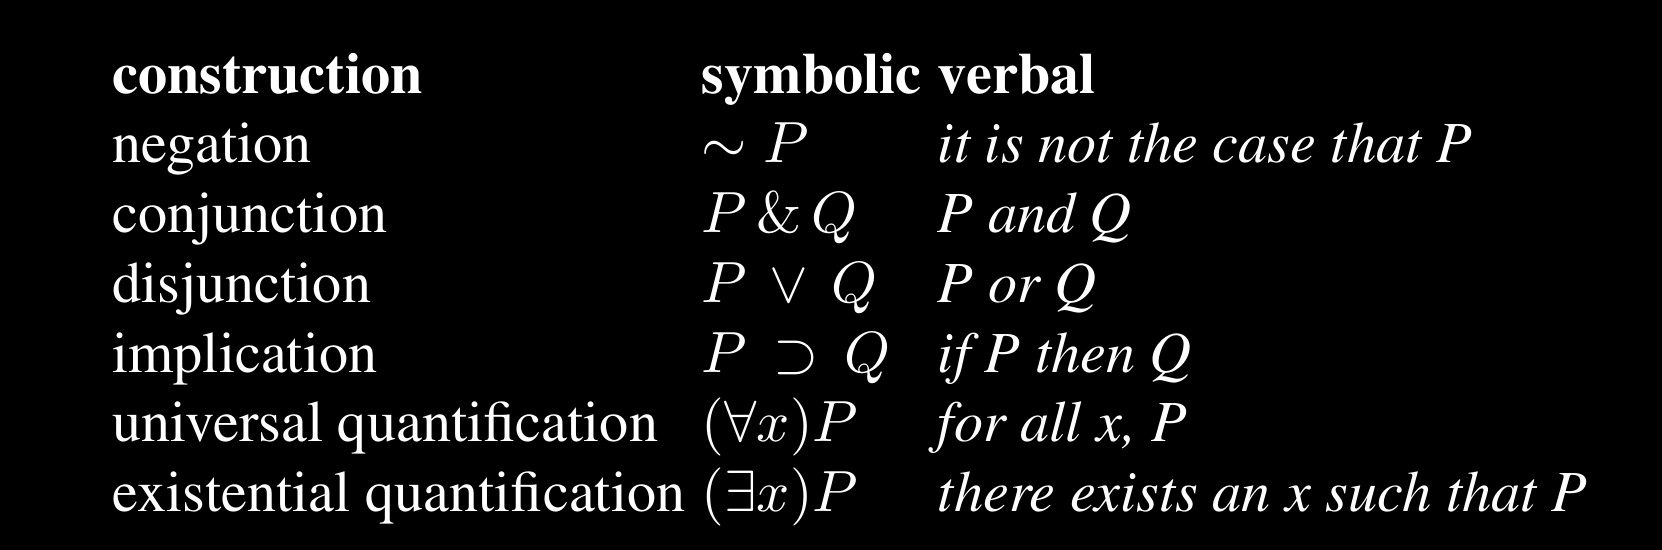
\includegraphics[width= \paperwidth]{core.png}
\end{figure}

\end{frame}

\begin{frame}
\frametitle{Extended Properties}

\begin{block}{Extended}
\begin{itemize}
\item Much more expressive
\item Semantically adequate
\item increases both number of categories and functions
\item also need for more complicated linearization categories
\item complex PGF backend to keep this syntactically complete
\item questions about scalability
\end{itemize}

\end{block}

\begin{exampleblock}{Extended Example}
\begin{itemize}
\item $\forall x (Nat(x) \supset Even(x) \lor Odd(x))$
\item ``every natural number is even or odd"
\end{itemize}
\end{exampleblock}

\end{frame}

\begin{frame}
\frametitle{Extended Syntax}

\begin{figure}
\hspace*{-3mm}%
   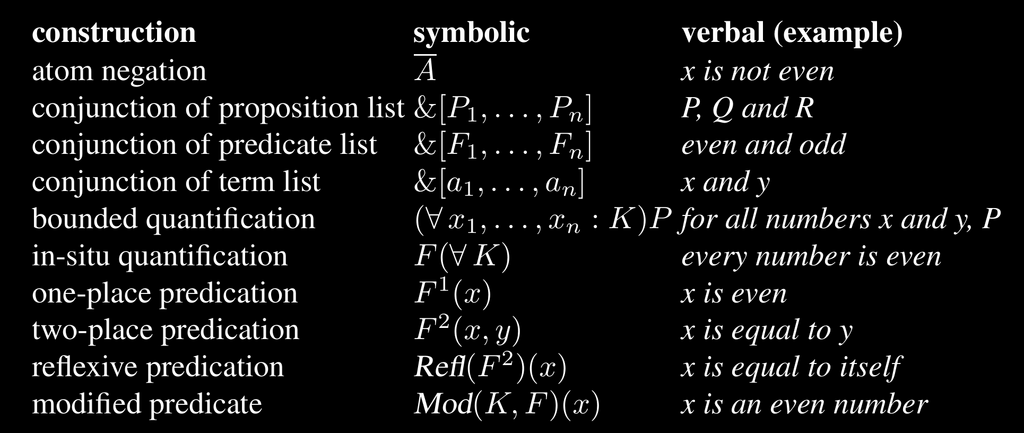
\includegraphics[width= \paperwidth]{e.png}
\end{figure}
\end{frame}


\begin{frame}
\frametitle{Translating to Core}
$\llbracket - \rrbracket : Extended \to Core$

\begin{itemize}
\item Core syntax as a model for extended
\item relatively simple in the sense that it is be deterministic
\item More or less uses the same logical structure from the ``standard view"
\end{itemize}
\end{frame}

\begin{frame}
\frametitle{Translating to Extended}

$\llbracket - \rrbracket : Core \to Extended$
\begin{itemize}
\item Difficult problem, infeasible at scale
\item Obscures formal detail, but is more intuitive 
\end{itemize}

\begin{exampleblock}{Conversion}
\begin{itemize}

\item Flattening a list \\
  $x\ and\ y\ and\ z\ \mapsto x,\ y\ and\ z$
\item Aggregation \\
  $x\ is\ even\ or\ x\ is\ odd\ \mapsto x\ is\ even\ or\ odd$
\item In-situ quantification \\
  $\forall\ n\ \in Nat,\ x\ is\ even\ or\ x\ is\ odd \mapsto every\ Nat\ is\ even\ or \odd$
\item Negation \\
  $it\ is\ not\ that\ case\ that\ x\ is\ even\ \mapsto \x is\ not\ even$
\item Reflexivitazion \\
  $x\ is\ equal\ to\ x\ \mapsto x\ is\ equal\ to\ itself$
\item Modification \\
  $x\ is\ a\ number\ and\ x\ is\ even\ \mapsto x\ is\ an\ even\ number$
\end{itemize}
\end{exampleblock}
\end{frame}


\subsection{Hott '14}

\begin{frame}
\frametitle{An Unpublished Talk at the Stockholm University Math Seminar}

\begin{itemize}
\item Ranta, \emph{Translating Homotopy Type Theory in Grammatical Framework},
  Fall 2014
\item Case study for text of \emph{real} mathematics writing
\item Purely GF translation
\item Complex abstract structure including latex, metadocument structure, etc.
\item HoTT specific lexicon
\item Includes proofs, but AST not similar to PL
\item Includes both expressions and propositions (breaks Curry-Howard)
\item \emph{Semantically adequate}
\item \emph{Syntactically incomplete}
\end{itemize}
\end{frame}

\begin{frame}
\frametitle{HoTT Grammar Modules}

\begin{figure}
\hspace*{-3mm}%
   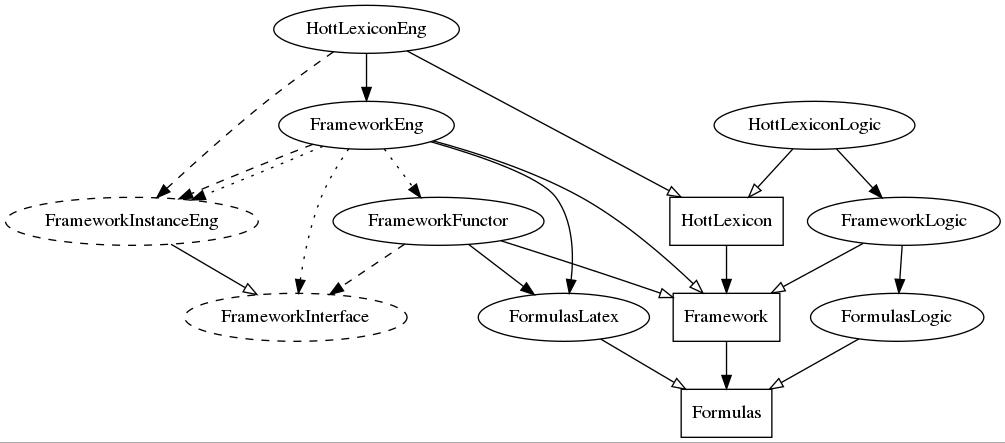
\includegraphics[width= \paperwidth]{testdep3.jpg}
\end{figure}
\end{frame}

\begin{frame}[fragile]
\frametitle{Framework.gf}
\begin{verbatim}
cat
  Paragraph ; -- definition, theorem, etc
  Definition ; -- definition of a new concept
  Assumption ; -- assumption in a proof -- let ...
  [Assumption]{1} ;  -- list of assumptions in one sentence
  Conclusion ; -- conclusion in a proof -- thus P
  Prop ; -- proposition,sentence or formula, A is contractible
  Sort ; -- set, type, etc corresponding to a common noun
  Ind ; -- individual element corresponding to a singular term
  Fun ; -- function with individual value
  Pred ; -- predicate: function with proposition value
  [Ind] ; -- list of individual expressions -- 1, 2 and 3
  UnivPhrase ; -- universal noun phrase -- for all x,y : A
  ConclusionPhrase ; -- conclusion word -- hence
  Label ; -- name/number of definition, theorem, etc
  Title ; -- title for theorem, definition, etc
\end{verbatim}
\end{frame}
\begin{frame}[fragile]

\frametitle{Formulas.gf}
\begin{verbatim}
cat
  Exp ;          -- formal expression             
                 -- x + y = z
  Var ;          -- variable
                 -- x
  [Var]{1} ;     -- list of variables             
                 -- x, y, z
  [Exp]{1} ;     -- list of expressions           
                 -- 1_{A}, A
  Format ;       -- line other than content       
                 -- \begin{document}
  MathEnv ;      -- math environment              
                 -- $ ... $
\end{verbatim}
\end{frame}

\begin{frame}[fragile]
\frametitle{Contractability}

\begin{block}{Comments}
\begin{itemize}
\item We work with the definition of contractability, the notion that a type (or space) is
actually a point, i.e. up to equality, there is only object
\item We show the (i) rendered latex, (ii)  pidgin Agda syntax after some concrete
  modifications, and (iii) the Agda code
\end{itemize}\\~\\
\end{block}

\textbf{Definition}:
A type $A$ is contractible, if there is $a : A$, called the center of contraction, such that for all $x : A$, $\equalH {a}{x}$.

\\~\\
\begin{figure}
\begin{verbatim}
isContr ( A : Set ) : Set = 
  ( a : A ) ( * ) ( ( x : A ) -> Id ( a ) ( x ) )
\end{verbatim}
\end{figure}

% 
\begin{code}[hide]%
\>[0]\AgdaSymbol{\{-\#}\AgdaSpace{}%
\AgdaKeyword{OPTIONS}\AgdaSpace{}%
\AgdaPragma{--omega-in-omega}\AgdaSpace{}%
\AgdaPragma{--type-in-type}\AgdaSpace{}%
\AgdaSymbol{\#-\}}\<%
\\
%
\\[\AgdaEmptyExtraSkip]%
\>[0]\AgdaKeyword{module}\AgdaSpace{}%
\AgdaModule{contr}\AgdaSpace{}%
\AgdaKeyword{where}\<%
\\
%
\\[\AgdaEmptyExtraSkip]%
\>[0]\AgdaKeyword{open}\AgdaSpace{}%
\AgdaKeyword{import}\AgdaSpace{}%
\AgdaModule{Agda.Builtin.Sigma}\AgdaSpace{}%
\AgdaKeyword{public}\<%
\\
%
\\[\AgdaEmptyExtraSkip]%
\>[0]\AgdaKeyword{variable}\<%
\\
\>[0][@{}l@{\AgdaIndent{0}}]%
\>[2]\AgdaGeneralizable{A}\AgdaSpace{}%
\AgdaGeneralizable{B}\AgdaSpace{}%
\AgdaSymbol{:}\AgdaSpace{}%
\AgdaPrimitive{Set}\<%
\\
%
\\[\AgdaEmptyExtraSkip]%
\>[0]\AgdaKeyword{data}\AgdaSpace{}%
\AgdaOperator{\AgdaDatatype{\AgdaUnderscore{}≡\AgdaUnderscore{}}}\AgdaSpace{}%
\AgdaSymbol{\{}\AgdaBound{A}\AgdaSpace{}%
\AgdaSymbol{:}\AgdaSpace{}%
\AgdaPrimitive{Set}\AgdaSymbol{\}}\AgdaSpace{}%
\AgdaSymbol{(}\AgdaBound{a}\AgdaSpace{}%
\AgdaSymbol{:}\AgdaSpace{}%
\AgdaBound{A}\AgdaSymbol{)}\AgdaSpace{}%
\AgdaSymbol{:}\AgdaSpace{}%
\AgdaBound{A}\AgdaSpace{}%
\AgdaSymbol{→}\AgdaSpace{}%
\AgdaPrimitive{Set}\AgdaSpace{}%
\AgdaKeyword{where}\<%
\\
\>[0][@{}l@{\AgdaIndent{0}}]%
\>[2]\AgdaInductiveConstructor{r}\AgdaSpace{}%
\AgdaSymbol{:}\AgdaSpace{}%
\AgdaBound{a}\AgdaSpace{}%
\AgdaOperator{\AgdaDatatype{≡}}\AgdaSpace{}%
\AgdaBound{a}\<%
\\
%
\\[\AgdaEmptyExtraSkip]%
\>[0]\AgdaKeyword{infix}\AgdaSpace{}%
\AgdaNumber{20}\AgdaSpace{}%
\AgdaOperator{\AgdaDatatype{\AgdaUnderscore{}≡\AgdaUnderscore{}}}\<%
\\
%
\\[\AgdaEmptyExtraSkip]%
\>[0]\AgdaFunction{id}\AgdaSpace{}%
\AgdaSymbol{:}\AgdaSpace{}%
\AgdaGeneralizable{A}\AgdaSpace{}%
\AgdaSymbol{→}\AgdaSpace{}%
\AgdaGeneralizable{A}\<%
\\
\>[0]\AgdaFunction{id}\AgdaSpace{}%
\AgdaSymbol{=}\AgdaSpace{}%
\AgdaSymbol{λ}\AgdaSpace{}%
\AgdaBound{z}\AgdaSpace{}%
\AgdaSymbol{→}\AgdaSpace{}%
\AgdaBound{z}\<%
\\
%
\\[\AgdaEmptyExtraSkip]%
\>[0]\<%
\end{code}

\begin{code}%
\>[0]\<%
\\
\>[0]\AgdaFunction{isContr}\AgdaSpace{}%
\AgdaSymbol{:}\AgdaSpace{}%
\AgdaSymbol{(}\AgdaBound{A}\AgdaSpace{}%
\AgdaSymbol{:}\AgdaSpace{}%
\AgdaPrimitive{Set}\AgdaSymbol{)}\AgdaSpace{}%
\AgdaSymbol{→}\AgdaSpace{}%
\AgdaPrimitive{Set}\<%
\\
\>[0]\AgdaFunction{isContr}\AgdaSpace{}%
\AgdaBound{A}\AgdaSpace{}%
\AgdaSymbol{=}%
\>[13]\AgdaRecord{Σ}\AgdaSpace{}%
\AgdaBound{A}\AgdaSpace{}%
\AgdaSymbol{λ}\AgdaSpace{}%
\AgdaBound{a}\AgdaSpace{}%
\AgdaSymbol{→}\AgdaSpace{}%
\AgdaSymbol{(}\AgdaBound{x}\AgdaSpace{}%
\AgdaSymbol{:}\AgdaSpace{}%
\AgdaBound{A}\AgdaSymbol{)}\AgdaSpace{}%
\AgdaSymbol{→}\AgdaSpace{}%
\AgdaSymbol{(}\AgdaBound{a}\AgdaSpace{}%
\AgdaOperator{\AgdaDatatype{≡}}\AgdaSpace{}%
\AgdaBound{x}\AgdaSymbol{)}\<%
\\
%
\\[\AgdaEmptyExtraSkip]%
\>[0]\<%
\end{code}


\end{frame}

\begin{frame}[fragile]
\frametitle{Equivalence}
\begin{itemize}
\item We also show that a notion of a map being an equivalence, that of the
  every element in the codomain having a contractible image (think bijection) 
\item notice the error in the Pidgin case
\end{itemize}

\\~\\

 \textbf{Definition}:
 A map $f : \arrowH {A}{B}$ is an equivalence, if for all $y : B$, its fiber, $\comprehensionH {x}{A}{\equalH {\appH {f}{x}}{y}}$, is contractible.
 We write $\equivalenceH {A}{B}$, if there is an equivalence $\arrowH {A}{B}$.


\begin{figure}
\begin{verbatim}
Equivalence ( f : A -> B ) : Set = 
  ( y : B ) -> ( isContr ( fiber it ) ) ; ; ; 
  fiber it : Set = ( x : A ) ( * ) ( Id ( f ( x ) ) ( y ) )
\end{verbatim}
\end{figure}

% 
\begin{code}[hide]%
\>[0]\AgdaSymbol{\{-\#}\AgdaSpace{}%
\AgdaKeyword{OPTIONS}\AgdaSpace{}%
\AgdaPragma{--omega-in-omega}\AgdaSpace{}%
\AgdaPragma{--type-in-type}\AgdaSpace{}%
\AgdaSymbol{\#-\}}\<%
\\
%
\\[\AgdaEmptyExtraSkip]%
\>[0]\AgdaKeyword{module}\AgdaSpace{}%
\AgdaModule{equiv}\AgdaSpace{}%
\AgdaKeyword{where}\<%
\\
%
\\[\AgdaEmptyExtraSkip]%
\>[0]\AgdaKeyword{open}\AgdaSpace{}%
\AgdaKeyword{import}\AgdaSpace{}%
\AgdaModule{Agda.Builtin.Sigma}\AgdaSpace{}%
\AgdaKeyword{public}\<%
\\
%
\\[\AgdaEmptyExtraSkip]%
\>[0]\AgdaKeyword{variable}\<%
\\
\>[0][@{}l@{\AgdaIndent{0}}]%
\>[2]\AgdaGeneralizable{A}\AgdaSpace{}%
\AgdaGeneralizable{B}\AgdaSpace{}%
\AgdaSymbol{:}\AgdaSpace{}%
\AgdaPrimitive{Set}\<%
\\
%
\\[\AgdaEmptyExtraSkip]%
\>[0]\AgdaKeyword{data}\AgdaSpace{}%
\AgdaOperator{\AgdaDatatype{\AgdaUnderscore{}≡\AgdaUnderscore{}}}\AgdaSpace{}%
\AgdaSymbol{\{}\AgdaBound{A}\AgdaSpace{}%
\AgdaSymbol{:}\AgdaSpace{}%
\AgdaPrimitive{Set}\AgdaSymbol{\}}\AgdaSpace{}%
\AgdaSymbol{(}\AgdaBound{a}\AgdaSpace{}%
\AgdaSymbol{:}\AgdaSpace{}%
\AgdaBound{A}\AgdaSymbol{)}\AgdaSpace{}%
\AgdaSymbol{:}\AgdaSpace{}%
\AgdaBound{A}\AgdaSpace{}%
\AgdaSymbol{→}\AgdaSpace{}%
\AgdaPrimitive{Set}\AgdaSpace{}%
\AgdaKeyword{where}\<%
\\
\>[0][@{}l@{\AgdaIndent{0}}]%
\>[2]\AgdaInductiveConstructor{r}\AgdaSpace{}%
\AgdaSymbol{:}\AgdaSpace{}%
\AgdaBound{a}\AgdaSpace{}%
\AgdaOperator{\AgdaDatatype{≡}}\AgdaSpace{}%
\AgdaBound{a}\<%
\\
%
\\[\AgdaEmptyExtraSkip]%
\>[0]\AgdaKeyword{infix}\AgdaSpace{}%
\AgdaNumber{20}\AgdaSpace{}%
\AgdaOperator{\AgdaDatatype{\AgdaUnderscore{}≡\AgdaUnderscore{}}}\<%
\\
%
\\[\AgdaEmptyExtraSkip]%
\>[0]\AgdaFunction{id}\AgdaSpace{}%
\AgdaSymbol{:}\AgdaSpace{}%
\AgdaGeneralizable{A}\AgdaSpace{}%
\AgdaSymbol{→}\AgdaSpace{}%
\AgdaGeneralizable{A}\<%
\\
\>[0]\AgdaFunction{id}\AgdaSpace{}%
\AgdaSymbol{=}\AgdaSpace{}%
\AgdaSymbol{λ}\AgdaSpace{}%
\AgdaBound{z}\AgdaSpace{}%
\AgdaSymbol{→}\AgdaSpace{}%
\AgdaBound{z}\<%
\\
%
\\[\AgdaEmptyExtraSkip]%
\>[0]\AgdaFunction{isContr}\AgdaSpace{}%
\AgdaSymbol{:}\AgdaSpace{}%
\AgdaSymbol{(}\AgdaBound{A}\AgdaSpace{}%
\AgdaSymbol{:}\AgdaSpace{}%
\AgdaPrimitive{Set}\AgdaSymbol{)}\AgdaSpace{}%
\AgdaSymbol{→}\AgdaSpace{}%
\AgdaPrimitive{Set}\<%
\\
\>[0]\AgdaFunction{isContr}\AgdaSpace{}%
\AgdaBound{A}\AgdaSpace{}%
\AgdaSymbol{=}%
\>[13]\AgdaRecord{Σ}\AgdaSpace{}%
\AgdaBound{A}\AgdaSpace{}%
\AgdaSymbol{λ}\AgdaSpace{}%
\AgdaBound{a}\AgdaSpace{}%
\AgdaSymbol{→}\AgdaSpace{}%
\AgdaSymbol{(}\AgdaBound{x}\AgdaSpace{}%
\AgdaSymbol{:}\AgdaSpace{}%
\AgdaBound{A}\AgdaSymbol{)}\AgdaSpace{}%
\AgdaSymbol{→}\AgdaSpace{}%
\AgdaSymbol{(}\AgdaBound{a}\AgdaSpace{}%
\AgdaOperator{\AgdaDatatype{≡}}\AgdaSpace{}%
\AgdaBound{x}\AgdaSymbol{)}\<%
\\
\>[0]\<%
\end{code}

\begin{code}%
\>[0]\<%
\\
%
\\[\AgdaEmptyExtraSkip]%
\>[0]\AgdaFunction{Equivalence}\AgdaSpace{}%
\AgdaSymbol{:}\AgdaSpace{}%
\AgdaSymbol{(}\AgdaBound{A}\AgdaSpace{}%
\AgdaBound{B}\AgdaSpace{}%
\AgdaSymbol{:}\AgdaSpace{}%
\AgdaPrimitive{Set}\AgdaSymbol{)}\AgdaSpace{}%
\AgdaSymbol{→}\AgdaSpace{}%
\AgdaSymbol{(}\AgdaBound{f}\AgdaSpace{}%
\AgdaSymbol{:}\AgdaSpace{}%
\AgdaBound{A}\AgdaSpace{}%
\AgdaSymbol{→}\AgdaSpace{}%
\AgdaBound{B}\AgdaSymbol{)}\AgdaSpace{}%
\AgdaSymbol{→}\AgdaSpace{}%
\AgdaPrimitive{Set}\<%
\\
\>[0]\AgdaFunction{Equivalence}\AgdaSpace{}%
\AgdaBound{A}\AgdaSpace{}%
\AgdaBound{B}\AgdaSpace{}%
\AgdaBound{f}\AgdaSpace{}%
\AgdaSymbol{=}\AgdaSpace{}%
\AgdaSymbol{∀}\AgdaSpace{}%
\AgdaSymbol{(}\AgdaBound{y}\AgdaSpace{}%
\AgdaSymbol{:}\AgdaSpace{}%
\AgdaBound{B}\AgdaSymbol{)}\AgdaSpace{}%
\AgdaSymbol{→}\AgdaSpace{}%
\AgdaFunction{isContr}\AgdaSpace{}%
\AgdaSymbol{(}\AgdaFunction{fiber'}\AgdaSpace{}%
\AgdaBound{y}\AgdaSymbol{)}\<%
\\
\>[0][@{}l@{\AgdaIndent{0}}]%
\>[2]\AgdaKeyword{where}\<%
\\
\>[2][@{}l@{\AgdaIndent{0}}]%
\>[4]\AgdaFunction{fiber'}\AgdaSpace{}%
\AgdaSymbol{:}\AgdaSpace{}%
\AgdaSymbol{(}\AgdaBound{y}\AgdaSpace{}%
\AgdaSymbol{:}\AgdaSpace{}%
\AgdaBound{B}\AgdaSymbol{)}\AgdaSpace{}%
\AgdaSymbol{→}\AgdaSpace{}%
\AgdaPrimitive{Set}\<%
\\
%
\>[4]\AgdaFunction{fiber'}\AgdaSpace{}%
\AgdaBound{y}\AgdaSpace{}%
\AgdaSymbol{=}\AgdaSpace{}%
\AgdaRecord{Σ}\AgdaSpace{}%
\AgdaBound{A}\AgdaSpace{}%
\AgdaSymbol{(λ}\AgdaSpace{}%
\AgdaBound{x}\AgdaSpace{}%
\AgdaSymbol{→}\AgdaSpace{}%
\AgdaBound{y}\AgdaSpace{}%
\AgdaOperator{\AgdaDatatype{≡}}\AgdaSpace{}%
\AgdaBound{f}\AgdaSpace{}%
\AgdaBound{x}\AgdaSymbol{)}\<%
\\
\>[0]\<%
\end{code}

\end{frame}

\subsection{A PL in GF}

\begin{frame}
\frametitle{GF as a programming language parser}

\begin{itemize}
\item How can a PL parser be bootstrapped to linearize to natural language ?
\item \emph{Syntactically adequate} out the box
\item All precedence information at the concrete level
\item There exists many existing programs to test on, hopefully less
  overhead 
\item In dependently typed language, almost everything is an expression \\
\item No distinguishing syntactically between types and terms
\item This makes the \emph{abstract syntax} easy to write for the PL (in GF) but difficult for the NL
\item Caution : This also makes it difficult to implement an ITP
\end{itemize}
\end{frame}


\begin{frame}[fragile]
\frametitle{Basic Categories}
\begin{verbatim}
cat
  Exp ;
  Var ;
  Tele ;
  LTele ;
  [Var]{1} ;
  [Tele]{2} ;
  [LTele]{2} ;
  Decl ;

  --cat [C] {n}
  -- =
  --cat ListC ;
  --fun BaseC : C -> ...-> C -> ListC ; -- n C ’s
  --fun ConsC : C -> ListC -> ListC
\end{verbatim}
\end{frame}

\begin{frame}[fragile]

\frametitle{Dependent Lambda Calculus with Propositional Equality}

\begin{verbatim}
fun
  Dtype , Dterm : Var -> Exp -> Decl ; 

  Earr : Exp -> Exp -> Exp ;
  Epi : [Tele] -> Exp -> Exp ;
  Eid : Exp -> Exp -> Exp -> Exp ; -- for type
  Eid2 : Exp -> Exp -> Exp ;
  Enat , Euni : Exp ;

  Evar : Var -> Exp ;
  Elam : [LTele] -> Exp -> Exp ;
  Eapp : Exp -> Exp -> Exp ;

  Erefl : Exp ;
  Eidind : Exp -> Exp -> Exp -> Exp -> Exp -> Exp ;

  Ezer : Exp ;
  Esuc : Exp -> Exp ;
  EsucEta : Exp ; 
  Enatind : Exp -> Exp -> Exp -> Exp -> Exp ;
\end{verbatim}
\end{frame}


\begin{frame}
\frametitle{Natural Numbers in Agda}
% \begin{code}[hide]%
\>[0]\<%
\\
\>[0]\AgdaKeyword{module}\AgdaSpace{}%
\AgdaModule{n}\AgdaSpace{}%
\AgdaKeyword{where}\<%
\\
%
\\[\AgdaEmptyExtraSkip]%
\>[0]\AgdaKeyword{open}\AgdaSpace{}%
\AgdaKeyword{import}\AgdaSpace{}%
\AgdaModule{Agda.Builtin.Nat}\AgdaSpace{}%
\AgdaKeyword{renaming}\AgdaSpace{}%
\AgdaSymbol{(}\AgdaDatatype{Nat}\AgdaSpace{}%
\AgdaSymbol{to}\AgdaSpace{}%
\AgdaDatatype{ℕ}\AgdaSymbol{)}\AgdaSpace{}%
\AgdaKeyword{public}\<%
\\
\>[0]\AgdaKeyword{import}\AgdaSpace{}%
\AgdaModule{Relation.Binary.PropositionalEquality}\AgdaSpace{}%
\AgdaSymbol{as}\AgdaSpace{}%
\AgdaModule{Eq}\<%
\\
\>[0]\AgdaKeyword{open}\AgdaSpace{}%
\AgdaModule{Eq}\AgdaSpace{}%
\AgdaKeyword{using}\AgdaSpace{}%
\AgdaSymbol{(}\AgdaOperator{\AgdaDatatype{\AgdaUnderscore{}≡\AgdaUnderscore{}}}\AgdaSymbol{;}\AgdaSpace{}%
\AgdaInductiveConstructor{refl}\AgdaSymbol{;}\AgdaSpace{}%
\AgdaFunction{trans}\AgdaSymbol{;}\AgdaSpace{}%
\AgdaFunction{sym}\AgdaSymbol{;}\AgdaSpace{}%
\AgdaFunction{cong}\AgdaSymbol{;}\AgdaSpace{}%
\AgdaFunction{cong-app}\AgdaSymbol{;}\AgdaSpace{}%
\AgdaFunction{subst}\AgdaSymbol{)}\<%
\\
\>[0]\AgdaKeyword{open}\AgdaSpace{}%
\AgdaModule{Eq.≡-Reasoning}\AgdaSpace{}%
\AgdaKeyword{using}\AgdaSpace{}%
\AgdaSymbol{(}\AgdaOperator{\AgdaFunction{begin\AgdaUnderscore{}}}\AgdaSymbol{;}\AgdaSpace{}%
\AgdaOperator{\AgdaFunction{\AgdaUnderscore{}≡⟨⟩\AgdaUnderscore{}}}\AgdaSymbol{;}\AgdaSpace{}%
\AgdaFunction{step-≡}\AgdaSymbol{;}\AgdaSpace{}%
\AgdaOperator{\AgdaFunction{\AgdaUnderscore{}∎}}\AgdaSymbol{)}\<%
\\
%
\\[\AgdaEmptyExtraSkip]%
\>[0]\AgdaKeyword{variable}\<%
\\
\>[0][@{}l@{\AgdaIndent{0}}]%
\>[2]\AgdaGeneralizable{A}\AgdaSpace{}%
\AgdaGeneralizable{B}\AgdaSpace{}%
\AgdaSymbol{:}\AgdaSpace{}%
\AgdaPrimitive{Set}\<%
\\
%
\>[2]\AgdaGeneralizable{a}\AgdaSpace{}%
\AgdaGeneralizable{a'}\AgdaSpace{}%
\AgdaSymbol{:}\AgdaSpace{}%
\AgdaGeneralizable{A}\<%
\\
\>[0]\<%
\end{code}

\begin{code}%
\>[0]\AgdaKeyword{data}\AgdaSpace{}%
\AgdaDatatype{ℕ'}\AgdaSpace{}%
\AgdaSymbol{:}\AgdaSpace{}%
\AgdaPrimitive{Set}\AgdaSpace{}%
\AgdaKeyword{where}\<%
\\
\>[0][@{}l@{\AgdaIndent{0}}]%
\>[2]\AgdaInductiveConstructor{zero'}\AgdaSpace{}%
\AgdaSymbol{:}\AgdaSpace{}%
\AgdaDatatype{ℕ'}\<%
\\
%
\>[2]\AgdaInductiveConstructor{suc'}%
\>[8]\AgdaSymbol{:}\AgdaSpace{}%
\AgdaDatatype{ℕ'}\AgdaSpace{}%
\AgdaSymbol{→}\AgdaSpace{}%
\AgdaDatatype{ℕ'}\<%
\\
%
\\[\AgdaEmptyExtraSkip]%
\>[0]\AgdaKeyword{data}\AgdaSpace{}%
\AgdaOperator{\AgdaDatatype{\AgdaUnderscore{}≡'\AgdaUnderscore{}}}\AgdaSpace{}%
\AgdaSymbol{\{}\AgdaBound{A}\AgdaSpace{}%
\AgdaSymbol{:}\AgdaSpace{}%
\AgdaPrimitive{Set}\AgdaSymbol{\}}\AgdaSpace{}%
\AgdaSymbol{(}\AgdaBound{a}\AgdaSpace{}%
\AgdaSymbol{:}\AgdaSpace{}%
\AgdaBound{A}\AgdaSymbol{)}\AgdaSpace{}%
\AgdaSymbol{:}\AgdaSpace{}%
\AgdaBound{A}\AgdaSpace{}%
\AgdaSymbol{→}\AgdaSpace{}%
\AgdaPrimitive{Set}\AgdaSpace{}%
\AgdaKeyword{where}\<%
\\
\>[0][@{}l@{\AgdaIndent{0}}]%
\>[2]\AgdaInductiveConstructor{refl'}\AgdaSpace{}%
\AgdaSymbol{:}\AgdaSpace{}%
\AgdaBound{a}\AgdaSpace{}%
\AgdaOperator{\AgdaDatatype{≡'}}\AgdaSpace{}%
\AgdaBound{a}\<%
\\
%
\\[\AgdaEmptyExtraSkip]%
\>[0]\AgdaFunction{two}\AgdaSpace{}%
\AgdaSymbol{:}\AgdaSpace{}%
\AgdaDatatype{ℕ'}\<%
\\
\>[0]\AgdaFunction{two}\AgdaSpace{}%
\AgdaSymbol{=}\AgdaSpace{}%
\AgdaInductiveConstructor{suc'}\AgdaSpace{}%
\AgdaSymbol{(}\AgdaInductiveConstructor{suc'}\AgdaSpace{}%
\AgdaInductiveConstructor{zero'}\AgdaSymbol{)}\<%
\\
%
\\[\AgdaEmptyExtraSkip]%
\>[0]\AgdaFunction{double}\AgdaSpace{}%
\AgdaSymbol{:}\AgdaSpace{}%
\AgdaDatatype{ℕ'}\AgdaSpace{}%
\AgdaSymbol{→}\AgdaSpace{}%
\AgdaDatatype{ℕ'}\<%
\\
\>[0]\AgdaFunction{double}\AgdaSpace{}%
\AgdaInductiveConstructor{zero'}\AgdaSpace{}%
\AgdaSymbol{=}\AgdaSpace{}%
\AgdaInductiveConstructor{zero'}\<%
\\
\>[0]\AgdaFunction{double}\AgdaSpace{}%
\AgdaSymbol{(}\AgdaInductiveConstructor{suc'}\AgdaSpace{}%
\AgdaBound{n}\AgdaSymbol{)}\AgdaSpace{}%
\AgdaSymbol{=}\AgdaSpace{}%
\AgdaInductiveConstructor{suc'}\AgdaSpace{}%
\AgdaSymbol{(}\AgdaInductiveConstructor{suc'}\AgdaSpace{}%
\AgdaSymbol{(}\AgdaFunction{double}\AgdaSpace{}%
\AgdaBound{n}\AgdaSymbol{))}\<%
\\
%
\\[\AgdaEmptyExtraSkip]%
\>[0]\AgdaFunction{four}\AgdaSpace{}%
\AgdaSymbol{:}\AgdaSpace{}%
\AgdaDatatype{ℕ'}\<%
\\
\>[0]\AgdaFunction{four}\AgdaSpace{}%
\AgdaSymbol{=}\AgdaSpace{}%
\AgdaFunction{double}\AgdaSpace{}%
\AgdaFunction{two}\<%
\\
%
\\[\AgdaEmptyExtraSkip]%
\>[0]\AgdaOperator{\AgdaFunction{\AgdaUnderscore{}+'\AgdaUnderscore{}}}\AgdaSpace{}%
\AgdaSymbol{:}\AgdaSpace{}%
\AgdaDatatype{ℕ'}\AgdaSpace{}%
\AgdaSymbol{→}\AgdaSpace{}%
\AgdaDatatype{ℕ'}\AgdaSpace{}%
\AgdaSymbol{→}\AgdaSpace{}%
\AgdaDatatype{ℕ'}\<%
\\
\>[0]\AgdaInductiveConstructor{zero'}\AgdaSpace{}%
\AgdaOperator{\AgdaFunction{+'}}\AgdaSpace{}%
\AgdaBound{y}\AgdaSpace{}%
\AgdaSymbol{=}\AgdaSpace{}%
\AgdaBound{y}\<%
\\
\>[0]\AgdaInductiveConstructor{suc'}\AgdaSpace{}%
\AgdaBound{x}\AgdaSpace{}%
\AgdaOperator{\AgdaFunction{+'}}\AgdaSpace{}%
\AgdaBound{y}\AgdaSpace{}%
\AgdaSymbol{=}\AgdaSpace{}%
\AgdaInductiveConstructor{suc'}\AgdaSpace{}%
\AgdaSymbol{(}\AgdaBound{x}\AgdaSpace{}%
\AgdaOperator{\AgdaFunction{+'}}\AgdaSpace{}%
\AgdaBound{y}\AgdaSymbol{)}\<%
\\
%
\\[\AgdaEmptyExtraSkip]%
\>[0]\AgdaFunction{2+2=4}\AgdaSpace{}%
\AgdaSymbol{:}\AgdaSpace{}%
\AgdaSymbol{(}\AgdaFunction{two}\AgdaSpace{}%
\AgdaOperator{\AgdaFunction{+'}}\AgdaSpace{}%
\AgdaFunction{two}\AgdaSymbol{)}\AgdaSpace{}%
\AgdaOperator{\AgdaDatatype{≡}}\AgdaSpace{}%
\AgdaFunction{four}\<%
\\
\>[0]\AgdaFunction{2+2=4}\AgdaSpace{}%
\AgdaSymbol{=}\AgdaSpace{}%
\AgdaInductiveConstructor{refl}\<%
\\
\>[0]\<%
\end{code}

\begin{code}[hide]%
\>[0]\<%
\\
\>[0]\AgdaFunction{ap}\AgdaSpace{}%
\AgdaSymbol{:}\AgdaSpace{}%
\AgdaSymbol{(}\AgdaBound{f}\AgdaSpace{}%
\AgdaSymbol{:}\AgdaSpace{}%
\AgdaGeneralizable{A}\AgdaSpace{}%
\AgdaSymbol{→}\AgdaSpace{}%
\AgdaGeneralizable{B}\AgdaSymbol{)}\AgdaSpace{}%
\AgdaSymbol{→}\AgdaSpace{}%
\AgdaGeneralizable{a}\AgdaSpace{}%
\AgdaOperator{\AgdaDatatype{≡}}\AgdaSpace{}%
\AgdaGeneralizable{a'}\AgdaSpace{}%
\AgdaSymbol{→}\AgdaSpace{}%
\AgdaBound{f}\AgdaSpace{}%
\AgdaGeneralizable{a}\AgdaSpace{}%
\AgdaOperator{\AgdaDatatype{≡}}\AgdaSpace{}%
\AgdaBound{f}\AgdaSpace{}%
\AgdaGeneralizable{a'}\<%
\\
\>[0]\AgdaFunction{ap}\AgdaSpace{}%
\AgdaBound{f}\AgdaSpace{}%
\AgdaInductiveConstructor{refl}\AgdaSpace{}%
\AgdaSymbol{=}\AgdaSpace{}%
\AgdaInductiveConstructor{refl}\<%
\\
%
\\[\AgdaEmptyExtraSkip]%
\>[0]\AgdaFunction{associativity-plus}\AgdaSpace{}%
\AgdaSymbol{:}\AgdaSpace{}%
\AgdaSymbol{(}\AgdaBound{m}\AgdaSpace{}%
\AgdaBound{n}\AgdaSpace{}%
\AgdaBound{p}\AgdaSpace{}%
\AgdaSymbol{:}\AgdaSpace{}%
\AgdaDatatype{ℕ}\AgdaSymbol{)}\AgdaSpace{}%
\AgdaSymbol{→}\AgdaSpace{}%
\AgdaSymbol{(}\AgdaSpace{}%
\AgdaSymbol{(}\AgdaSpace{}%
\AgdaBound{m}\AgdaSpace{}%
\AgdaOperator{\AgdaPrimitive{+}}\AgdaSpace{}%
\AgdaBound{n}\AgdaSpace{}%
\AgdaSymbol{)}\AgdaSpace{}%
\AgdaOperator{\AgdaPrimitive{+}}\AgdaSpace{}%
\AgdaBound{p}\AgdaSpace{}%
\AgdaSymbol{)}\AgdaSpace{}%
\AgdaOperator{\AgdaDatatype{≡}}\AgdaSpace{}%
\AgdaSymbol{(}\AgdaSpace{}%
\AgdaBound{m}\AgdaSpace{}%
\AgdaOperator{\AgdaPrimitive{+}}\AgdaSpace{}%
\AgdaSymbol{(}\AgdaSpace{}%
\AgdaBound{n}\AgdaSpace{}%
\AgdaOperator{\AgdaPrimitive{+}}\AgdaSpace{}%
\AgdaBound{p}\AgdaSpace{}%
\AgdaSymbol{)}\AgdaSpace{}%
\AgdaSymbol{)}\<%
\\
\>[0]\AgdaFunction{associativity-plus}\AgdaSpace{}%
\AgdaInductiveConstructor{zero}\AgdaSpace{}%
\AgdaBound{n}\AgdaSpace{}%
\AgdaBound{p}\AgdaSpace{}%
\AgdaSymbol{=}\AgdaSpace{}%
\AgdaInductiveConstructor{refl}\<%
\\
\>[0]\AgdaFunction{associativity-plus}\AgdaSpace{}%
\AgdaSymbol{(}\AgdaInductiveConstructor{suc}\AgdaSpace{}%
\AgdaBound{m}\AgdaSymbol{)}\AgdaSpace{}%
\AgdaBound{n}\AgdaSpace{}%
\AgdaBound{p}\AgdaSpace{}%
\AgdaSymbol{=}\AgdaSpace{}%
\AgdaFunction{ap}\AgdaSpace{}%
\AgdaInductiveConstructor{suc}\AgdaSpace{}%
\AgdaSymbol{(}\AgdaFunction{associativity-plus}\AgdaSpace{}%
\AgdaBound{m}\AgdaSpace{}%
\AgdaBound{n}\AgdaSpace{}%
\AgdaBound{p}\AgdaSymbol{)}\<%
\\
%
\\[\AgdaEmptyExtraSkip]%
\>[0]\AgdaFunction{natind}\AgdaSpace{}%
\AgdaSymbol{:}%
\>[172I]\AgdaSymbol{\{}\AgdaBound{C}\AgdaSpace{}%
\AgdaSymbol{:}\AgdaSpace{}%
\AgdaDatatype{ℕ}\AgdaSpace{}%
\AgdaSymbol{->}\AgdaSpace{}%
\AgdaPrimitive{Set}\AgdaSymbol{\}}\AgdaSpace{}%
\AgdaSymbol{->}%
\>[42]\AgdaComment{-- predicate}\<%
\\
\>[.][@{}l@{}]\<[172I]%
\>[9]\AgdaBound{C}\AgdaSpace{}%
\AgdaInductiveConstructor{zero}\AgdaSpace{}%
\AgdaSymbol{->}%
\>[42]\AgdaComment{-- base case}\<%
\\
%
\>[9]\AgdaSymbol{((}\AgdaBound{n}\AgdaSpace{}%
\AgdaSymbol{:}\AgdaSpace{}%
\AgdaDatatype{ℕ}\AgdaSymbol{)}\AgdaSpace{}%
\AgdaSymbol{->}\AgdaSpace{}%
\AgdaBound{C}\AgdaSpace{}%
\AgdaBound{n}\AgdaSpace{}%
\AgdaSymbol{->}\AgdaSpace{}%
\AgdaBound{C}\AgdaSpace{}%
\AgdaSymbol{(}\AgdaInductiveConstructor{suc}\AgdaSpace{}%
\AgdaBound{n}\AgdaSymbol{))}\AgdaSpace{}%
\AgdaSymbol{->}\AgdaSpace{}%
\AgdaComment{--IH}\<%
\\
%
\>[9]\AgdaSymbol{(}\AgdaBound{n}\AgdaSpace{}%
\AgdaSymbol{:}\AgdaSpace{}%
\AgdaDatatype{ℕ}\AgdaSymbol{)}\AgdaSpace{}%
\AgdaSymbol{->}\AgdaSpace{}%
\AgdaBound{C}\AgdaSpace{}%
\AgdaBound{n}\<%
\\
\>[0]\AgdaFunction{natind}\AgdaSpace{}%
\AgdaBound{base}\AgdaSpace{}%
\AgdaBound{step}\AgdaSpace{}%
\AgdaInductiveConstructor{zero}%
\>[26]\AgdaSymbol{=}\AgdaSpace{}%
\AgdaBound{base}\<%
\\
\>[0]\AgdaFunction{natind}\AgdaSpace{}%
\AgdaBound{base}\AgdaSpace{}%
\AgdaBound{step}\AgdaSpace{}%
\AgdaSymbol{(}\AgdaInductiveConstructor{suc}\AgdaSpace{}%
\AgdaBound{n}\AgdaSymbol{)}\AgdaSpace{}%
\AgdaSymbol{=}\AgdaSpace{}%
\AgdaBound{step}\AgdaSpace{}%
\AgdaBound{n}\AgdaSpace{}%
\AgdaSymbol{(}\AgdaFunction{natind}\AgdaSpace{}%
\AgdaBound{base}\AgdaSpace{}%
\AgdaBound{step}\AgdaSpace{}%
\AgdaBound{n}\AgdaSymbol{)}\<%
\\
%
\\[\AgdaEmptyExtraSkip]%
\>[0]\AgdaFunction{associativity-plus-ind}\AgdaSpace{}%
\AgdaSymbol{:}\<%
\\
\>[0][@{}l@{\AgdaIndent{0}}]%
\>[2]\AgdaSymbol{(}\AgdaBound{m}\AgdaSpace{}%
\AgdaBound{n}\AgdaSpace{}%
\AgdaBound{p}\AgdaSpace{}%
\AgdaSymbol{:}\AgdaSpace{}%
\AgdaDatatype{ℕ}\AgdaSymbol{)}\AgdaSpace{}%
\AgdaSymbol{→}\<%
\\
%
\>[2]\AgdaSymbol{((}\AgdaBound{m}\AgdaSpace{}%
\AgdaOperator{\AgdaPrimitive{+}}\AgdaSpace{}%
\AgdaBound{n}\AgdaSymbol{)}\AgdaSpace{}%
\AgdaOperator{\AgdaPrimitive{+}}\AgdaSpace{}%
\AgdaBound{p}\AgdaSymbol{)}\AgdaSpace{}%
\AgdaOperator{\AgdaDatatype{≡}}\AgdaSpace{}%
\AgdaSymbol{(}\AgdaBound{m}\AgdaSpace{}%
\AgdaOperator{\AgdaPrimitive{+}}\AgdaSpace{}%
\AgdaSymbol{(}\AgdaBound{n}\AgdaSpace{}%
\AgdaOperator{\AgdaPrimitive{+}}\AgdaSpace{}%
\AgdaBound{p}\AgdaSymbol{))}\<%
\\
\>[0]\AgdaFunction{associativity-plus-ind}\AgdaSpace{}%
\AgdaBound{m}\AgdaSpace{}%
\AgdaBound{n}\AgdaSpace{}%
\AgdaBound{p}\AgdaSpace{}%
\AgdaSymbol{=}\<%
\\
\>[0][@{}l@{\AgdaIndent{0}}]%
\>[2]\AgdaFunction{natind}\<%
\\
\>[2][@{}l@{\AgdaIndent{0}}]%
\>[4]\AgdaFunction{baseCase}\<%
\\
%
\>[4]\AgdaSymbol{(λ}\AgdaSpace{}%
\AgdaBound{n₁}\AgdaSpace{}%
\AgdaBound{ih}\AgdaSpace{}%
\AgdaSymbol{→}\AgdaSpace{}%
\AgdaFunction{simpl}\AgdaSpace{}%
\AgdaBound{n₁}\AgdaSpace{}%
\AgdaSymbol{(}\AgdaFunction{indCase}\AgdaSpace{}%
\AgdaBound{n₁}\AgdaSpace{}%
\AgdaBound{ih}\AgdaSymbol{))}\<%
\\
%
\>[4]\AgdaBound{m}\<%
\\
%
\>[2]\AgdaKeyword{where}\<%
\\
\>[2][@{}l@{\AgdaIndent{0}}]%
\>[4]\AgdaFunction{baseCase}\AgdaSpace{}%
\AgdaSymbol{:}\AgdaSpace{}%
\AgdaSymbol{(}\AgdaInductiveConstructor{zero}\AgdaSpace{}%
\AgdaOperator{\AgdaPrimitive{+}}\AgdaSpace{}%
\AgdaBound{n}\AgdaSpace{}%
\AgdaOperator{\AgdaPrimitive{+}}\AgdaSpace{}%
\AgdaBound{p}\AgdaSymbol{)}\AgdaSpace{}%
\AgdaOperator{\AgdaDatatype{≡}}\AgdaSpace{}%
\AgdaSymbol{(}\AgdaInductiveConstructor{zero}\AgdaSpace{}%
\AgdaOperator{\AgdaPrimitive{+}}\AgdaSpace{}%
\AgdaSymbol{(}\AgdaBound{n}\AgdaSpace{}%
\AgdaOperator{\AgdaPrimitive{+}}\AgdaSpace{}%
\AgdaBound{p}\AgdaSymbol{))}\<%
\\
%
\>[4]\AgdaFunction{baseCase}\AgdaSpace{}%
\AgdaSymbol{=}\AgdaSpace{}%
\AgdaInductiveConstructor{refl}\<%
\\
%
\>[4]\AgdaFunction{indCase}\AgdaSpace{}%
\AgdaSymbol{:}%
\>[254I]\AgdaSymbol{(}\AgdaBound{n'}\AgdaSpace{}%
\AgdaSymbol{:}\AgdaSpace{}%
\AgdaDatatype{ℕ}\AgdaSymbol{)}\AgdaSpace{}%
\AgdaSymbol{→}\AgdaSpace{}%
\AgdaSymbol{(}\AgdaBound{n'}\AgdaSpace{}%
\AgdaOperator{\AgdaPrimitive{+}}\AgdaSpace{}%
\AgdaBound{n}\AgdaSpace{}%
\AgdaOperator{\AgdaPrimitive{+}}\AgdaSpace{}%
\AgdaBound{p}\AgdaSymbol{)}\AgdaSpace{}%
\AgdaOperator{\AgdaDatatype{≡}}\AgdaSpace{}%
\AgdaSymbol{(}\AgdaBound{n'}\AgdaSpace{}%
\AgdaOperator{\AgdaPrimitive{+}}\AgdaSpace{}%
\AgdaSymbol{(}\AgdaBound{n}\AgdaSpace{}%
\AgdaOperator{\AgdaPrimitive{+}}\AgdaSpace{}%
\AgdaBound{p}\AgdaSymbol{))}\AgdaSpace{}%
\AgdaSymbol{→}\<%
\\
\>[254I][@{}l@{\AgdaIndent{0}}]%
\>[16]\AgdaInductiveConstructor{suc}\AgdaSpace{}%
\AgdaSymbol{(}\AgdaBound{n'}\AgdaSpace{}%
\AgdaOperator{\AgdaPrimitive{+}}\AgdaSpace{}%
\AgdaBound{n}\AgdaSpace{}%
\AgdaOperator{\AgdaPrimitive{+}}\AgdaSpace{}%
\AgdaBound{p}\AgdaSymbol{)}\AgdaSpace{}%
\AgdaOperator{\AgdaDatatype{≡}}\AgdaSpace{}%
\AgdaInductiveConstructor{suc}\AgdaSpace{}%
\AgdaSymbol{(}\AgdaBound{n'}\AgdaSpace{}%
\AgdaOperator{\AgdaPrimitive{+}}\AgdaSpace{}%
\AgdaSymbol{(}\AgdaBound{n}\AgdaSpace{}%
\AgdaOperator{\AgdaPrimitive{+}}\AgdaSpace{}%
\AgdaBound{p}\AgdaSymbol{))}\<%
\\
%
\>[4]\AgdaFunction{indCase}\AgdaSpace{}%
\AgdaSymbol{=}\AgdaSpace{}%
\AgdaSymbol{(λ}\AgdaSpace{}%
\AgdaBound{n'}\AgdaSpace{}%
\AgdaBound{x}\AgdaSpace{}%
\AgdaSymbol{→}\AgdaSpace{}%
\AgdaFunction{ap}\AgdaSpace{}%
\AgdaInductiveConstructor{suc}\AgdaSpace{}%
\AgdaBound{x}\AgdaSpace{}%
\AgdaSymbol{)}\<%
\\
%
\>[4]\AgdaFunction{simpl}\AgdaSpace{}%
\AgdaSymbol{:}%
\>[292I]\AgdaSymbol{(}\AgdaBound{n'}\AgdaSpace{}%
\AgdaSymbol{:}\AgdaSpace{}%
\AgdaDatatype{ℕ}\AgdaSymbol{)}\<%
\\
\>[.][@{}l@{}]\<[292I]%
\>[12]\AgdaSymbol{→}\AgdaSpace{}%
\AgdaInductiveConstructor{suc}\AgdaSpace{}%
\AgdaSymbol{(}\AgdaBound{n'}\AgdaSpace{}%
\AgdaOperator{\AgdaPrimitive{+}}\AgdaSpace{}%
\AgdaBound{n}\AgdaSpace{}%
\AgdaOperator{\AgdaPrimitive{+}}\AgdaSpace{}%
\AgdaBound{p}\AgdaSymbol{)}\AgdaSpace{}%
\AgdaOperator{\AgdaDatatype{≡}}\AgdaSpace{}%
\AgdaInductiveConstructor{suc}\AgdaSpace{}%
\AgdaSymbol{(}\AgdaBound{n'}\AgdaSpace{}%
\AgdaOperator{\AgdaPrimitive{+}}\AgdaSpace{}%
\AgdaSymbol{(}\AgdaBound{n}\AgdaSpace{}%
\AgdaOperator{\AgdaPrimitive{+}}\AgdaSpace{}%
\AgdaBound{p}\AgdaSymbol{))}\<%
\\
%
\>[12]\AgdaSymbol{→}\AgdaSpace{}%
\AgdaSymbol{(}\AgdaInductiveConstructor{suc}\AgdaSpace{}%
\AgdaBound{n'}\AgdaSpace{}%
\AgdaOperator{\AgdaPrimitive{+}}\AgdaSpace{}%
\AgdaBound{n}\AgdaSpace{}%
\AgdaOperator{\AgdaPrimitive{+}}\AgdaSpace{}%
\AgdaBound{p}\AgdaSymbol{)}\AgdaSpace{}%
\AgdaOperator{\AgdaDatatype{≡}}\AgdaSpace{}%
\AgdaSymbol{(}\AgdaInductiveConstructor{suc}\AgdaSpace{}%
\AgdaBound{n'}\AgdaSpace{}%
\AgdaOperator{\AgdaPrimitive{+}}\AgdaSpace{}%
\AgdaSymbol{(}\AgdaBound{n}\AgdaSpace{}%
\AgdaOperator{\AgdaPrimitive{+}}\AgdaSpace{}%
\AgdaBound{p}\AgdaSymbol{))}\<%
\\
%
\>[4]\AgdaFunction{simpl}\AgdaSpace{}%
\AgdaBound{n'}\AgdaSpace{}%
\AgdaBound{x}\AgdaSpace{}%
\AgdaSymbol{=}\AgdaSpace{}%
\AgdaBound{x}\<%
\end{code}

\end{frame}

\begin{frame}[fragile]
\frametitle{Proof Associativity of Natural Numbers from \emph{Software Foundations}}
% [from software foundations]
\begin{verbatim}
Theorem: For any n, m and p,
  n + (m + p) = (n + m) + p.
Proof: By induction on n.
  First, suppose n = 0. We must show that
    0 + (m + p) = (0 + m) + p.
  This follows directly from the definition of +.
  Next, suppose n = S n', where
    n' + (m + p) = (n' + m) + p.
  We must now show that
    (S n') + (m + p) = ((S n') + m) + p.
  By the definition of +, this follows from
    S (n' + (m + p)) = S ((n' + m) + p),
  which is immediate from the induction hypothesis. Qed.
\end{verbatim}
\end{frame}

\begin{frame}
\frametitle{Pattern Matching Proofs in Agda}

% \begin{code}[hide]%
\>[0]\<%
\\
\>[0]\AgdaKeyword{module}\AgdaSpace{}%
\AgdaModule{p}\AgdaSpace{}%
\AgdaKeyword{where}\<%
\\
%
\\[\AgdaEmptyExtraSkip]%
\>[0]\AgdaKeyword{open}\AgdaSpace{}%
\AgdaKeyword{import}\AgdaSpace{}%
\AgdaModule{Agda.Builtin.Nat}\AgdaSpace{}%
\AgdaKeyword{renaming}\AgdaSpace{}%
\AgdaSymbol{(}\AgdaDatatype{Nat}\AgdaSpace{}%
\AgdaSymbol{to}\AgdaSpace{}%
\AgdaDatatype{ℕ}\AgdaSymbol{)}\AgdaSpace{}%
\AgdaKeyword{public}\<%
\\
\>[0]\AgdaKeyword{import}\AgdaSpace{}%
\AgdaModule{Relation.Binary.PropositionalEquality}\AgdaSpace{}%
\AgdaSymbol{as}\AgdaSpace{}%
\AgdaModule{Eq}\<%
\\
\>[0]\AgdaKeyword{open}\AgdaSpace{}%
\AgdaModule{Eq}\AgdaSpace{}%
\AgdaKeyword{using}\AgdaSpace{}%
\AgdaSymbol{(}\AgdaOperator{\AgdaDatatype{\AgdaUnderscore{}≡\AgdaUnderscore{}}}\AgdaSymbol{;}\AgdaSpace{}%
\AgdaInductiveConstructor{refl}\AgdaSymbol{;}\AgdaSpace{}%
\AgdaFunction{trans}\AgdaSymbol{;}\AgdaSpace{}%
\AgdaFunction{sym}\AgdaSymbol{;}\AgdaSpace{}%
\AgdaFunction{cong}\AgdaSymbol{;}\AgdaSpace{}%
\AgdaFunction{cong-app}\AgdaSymbol{;}\AgdaSpace{}%
\AgdaFunction{subst}\AgdaSymbol{)}\<%
\\
\>[0]\AgdaKeyword{open}\AgdaSpace{}%
\AgdaModule{Eq.≡-Reasoning}\AgdaSpace{}%
\AgdaKeyword{using}\AgdaSpace{}%
\AgdaSymbol{(}\AgdaOperator{\AgdaFunction{begin\AgdaUnderscore{}}}\AgdaSymbol{;}\AgdaSpace{}%
\AgdaOperator{\AgdaFunction{\AgdaUnderscore{}≡⟨⟩\AgdaUnderscore{}}}\AgdaSymbol{;}\AgdaSpace{}%
\AgdaFunction{step-≡}\AgdaSymbol{;}\AgdaSpace{}%
\AgdaOperator{\AgdaFunction{\AgdaUnderscore{}∎}}\AgdaSymbol{)}\<%
\\
%
\\[\AgdaEmptyExtraSkip]%
\>[0]\AgdaKeyword{variable}\<%
\\
\>[0][@{}l@{\AgdaIndent{0}}]%
\>[2]\AgdaGeneralizable{A}\AgdaSpace{}%
\AgdaGeneralizable{B}\AgdaSpace{}%
\AgdaSymbol{:}\AgdaSpace{}%
\AgdaPrimitive{Set}\<%
\\
%
\>[2]\AgdaGeneralizable{a}\AgdaSpace{}%
\AgdaGeneralizable{a'}\AgdaSpace{}%
\AgdaSymbol{:}\AgdaSpace{}%
\AgdaGeneralizable{A}\<%
\\
\>[0]\<%
\end{code}

\begin{code}[hide]%
\>[0]\AgdaKeyword{data}\AgdaSpace{}%
\AgdaDatatype{ℕ'}\AgdaSpace{}%
\AgdaSymbol{:}\AgdaSpace{}%
\AgdaPrimitive{Set}\AgdaSpace{}%
\AgdaKeyword{where}\<%
\\
\>[0][@{}l@{\AgdaIndent{0}}]%
\>[2]\AgdaInductiveConstructor{zero'}\AgdaSpace{}%
\AgdaSymbol{:}\AgdaSpace{}%
\AgdaDatatype{ℕ'}\<%
\\
%
\>[2]\AgdaInductiveConstructor{suc'}%
\>[8]\AgdaSymbol{:}\AgdaSpace{}%
\AgdaDatatype{ℕ'}\AgdaSpace{}%
\AgdaSymbol{→}\AgdaSpace{}%
\AgdaDatatype{ℕ'}\<%
\\
%
\\[\AgdaEmptyExtraSkip]%
\>[0]\AgdaKeyword{data}\AgdaSpace{}%
\AgdaOperator{\AgdaDatatype{\AgdaUnderscore{}≡'\AgdaUnderscore{}}}\AgdaSpace{}%
\AgdaSymbol{\{}\AgdaBound{A}\AgdaSpace{}%
\AgdaSymbol{:}\AgdaSpace{}%
\AgdaPrimitive{Set}\AgdaSymbol{\}}\AgdaSpace{}%
\AgdaSymbol{(}\AgdaBound{a}\AgdaSpace{}%
\AgdaSymbol{:}\AgdaSpace{}%
\AgdaBound{A}\AgdaSymbol{)}\AgdaSpace{}%
\AgdaSymbol{:}\AgdaSpace{}%
\AgdaBound{A}\AgdaSpace{}%
\AgdaSymbol{→}\AgdaSpace{}%
\AgdaPrimitive{Set}\AgdaSpace{}%
\AgdaKeyword{where}\<%
\\
\>[0][@{}l@{\AgdaIndent{0}}]%
\>[2]\AgdaInductiveConstructor{refl'}\AgdaSpace{}%
\AgdaSymbol{:}\AgdaSpace{}%
\AgdaBound{a}\AgdaSpace{}%
\AgdaOperator{\AgdaDatatype{≡'}}\AgdaSpace{}%
\AgdaBound{a}\<%
\\
%
\\[\AgdaEmptyExtraSkip]%
\>[0]\AgdaFunction{two}\AgdaSpace{}%
\AgdaSymbol{:}\AgdaSpace{}%
\AgdaDatatype{ℕ'}\<%
\\
\>[0]\AgdaFunction{two}\AgdaSpace{}%
\AgdaSymbol{=}\AgdaSpace{}%
\AgdaInductiveConstructor{suc'}\AgdaSpace{}%
\AgdaSymbol{(}\AgdaInductiveConstructor{suc'}\AgdaSpace{}%
\AgdaInductiveConstructor{zero'}\AgdaSymbol{)}\<%
\\
%
\\[\AgdaEmptyExtraSkip]%
\>[0]\AgdaFunction{double}\AgdaSpace{}%
\AgdaSymbol{:}\AgdaSpace{}%
\AgdaDatatype{ℕ'}\AgdaSpace{}%
\AgdaSymbol{→}\AgdaSpace{}%
\AgdaDatatype{ℕ'}\<%
\\
\>[0]\AgdaFunction{double}\AgdaSpace{}%
\AgdaInductiveConstructor{zero'}\AgdaSpace{}%
\AgdaSymbol{=}\AgdaSpace{}%
\AgdaInductiveConstructor{zero'}\<%
\\
\>[0]\AgdaFunction{double}\AgdaSpace{}%
\AgdaSymbol{(}\AgdaInductiveConstructor{suc'}\AgdaSpace{}%
\AgdaBound{n}\AgdaSymbol{)}\AgdaSpace{}%
\AgdaSymbol{=}\AgdaSpace{}%
\AgdaInductiveConstructor{suc'}\AgdaSpace{}%
\AgdaSymbol{(}\AgdaInductiveConstructor{suc'}\AgdaSpace{}%
\AgdaSymbol{(}\AgdaFunction{double}\AgdaSpace{}%
\AgdaBound{n}\AgdaSymbol{))}\<%
\\
%
\\[\AgdaEmptyExtraSkip]%
\>[0]\AgdaFunction{four}\AgdaSpace{}%
\AgdaSymbol{:}\AgdaSpace{}%
\AgdaDatatype{ℕ'}\<%
\\
\>[0]\AgdaFunction{four}\AgdaSpace{}%
\AgdaSymbol{=}\AgdaSpace{}%
\AgdaFunction{double}\AgdaSpace{}%
\AgdaFunction{two}\<%
\\
%
\\[\AgdaEmptyExtraSkip]%
\>[0]\AgdaOperator{\AgdaFunction{\AgdaUnderscore{}+'\AgdaUnderscore{}}}\AgdaSpace{}%
\AgdaSymbol{:}\AgdaSpace{}%
\AgdaDatatype{ℕ'}\AgdaSpace{}%
\AgdaSymbol{→}\AgdaSpace{}%
\AgdaDatatype{ℕ'}\AgdaSpace{}%
\AgdaSymbol{→}\AgdaSpace{}%
\AgdaDatatype{ℕ'}\<%
\\
\>[0]\AgdaInductiveConstructor{zero'}\AgdaSpace{}%
\AgdaOperator{\AgdaFunction{+'}}\AgdaSpace{}%
\AgdaBound{y}\AgdaSpace{}%
\AgdaSymbol{=}\AgdaSpace{}%
\AgdaBound{y}\<%
\\
\>[0]\AgdaInductiveConstructor{suc'}\AgdaSpace{}%
\AgdaBound{x}\AgdaSpace{}%
\AgdaOperator{\AgdaFunction{+'}}\AgdaSpace{}%
\AgdaBound{y}\AgdaSpace{}%
\AgdaSymbol{=}\AgdaSpace{}%
\AgdaInductiveConstructor{suc'}\AgdaSpace{}%
\AgdaSymbol{(}\AgdaBound{x}\AgdaSpace{}%
\AgdaOperator{\AgdaFunction{+'}}\AgdaSpace{}%
\AgdaBound{y}\AgdaSymbol{)}\<%
\\
%
\\[\AgdaEmptyExtraSkip]%
\>[0]\AgdaFunction{2+2=4}\AgdaSpace{}%
\AgdaSymbol{:}\AgdaSpace{}%
\AgdaSymbol{(}\AgdaFunction{two}\AgdaSpace{}%
\AgdaOperator{\AgdaFunction{+'}}\AgdaSpace{}%
\AgdaFunction{two}\AgdaSymbol{)}\AgdaSpace{}%
\AgdaOperator{\AgdaDatatype{≡}}\AgdaSpace{}%
\AgdaFunction{four}\<%
\\
\>[0]\AgdaFunction{2+2=4}\AgdaSpace{}%
\AgdaSymbol{=}\AgdaSpace{}%
\AgdaInductiveConstructor{refl}\<%
\\
\>[0]\<%
\end{code}

\begin{code}%
\>[0]\<%
\\
\>[0]\AgdaFunction{ap}\AgdaSpace{}%
\AgdaSymbol{:}\AgdaSpace{}%
\AgdaSymbol{(}\AgdaBound{f}\AgdaSpace{}%
\AgdaSymbol{:}\AgdaSpace{}%
\AgdaGeneralizable{A}\AgdaSpace{}%
\AgdaSymbol{→}\AgdaSpace{}%
\AgdaGeneralizable{B}\AgdaSymbol{)}\AgdaSpace{}%
\AgdaSymbol{→}\AgdaSpace{}%
\AgdaGeneralizable{a}\AgdaSpace{}%
\AgdaOperator{\AgdaDatatype{≡}}\AgdaSpace{}%
\AgdaGeneralizable{a'}\AgdaSpace{}%
\AgdaSymbol{→}\AgdaSpace{}%
\AgdaBound{f}\AgdaSpace{}%
\AgdaGeneralizable{a}\AgdaSpace{}%
\AgdaOperator{\AgdaDatatype{≡}}\AgdaSpace{}%
\AgdaBound{f}\AgdaSpace{}%
\AgdaGeneralizable{a'}\<%
\\
\>[0]\AgdaFunction{ap}\AgdaSpace{}%
\AgdaBound{f}\AgdaSpace{}%
\AgdaInductiveConstructor{refl}\AgdaSpace{}%
\AgdaSymbol{=}\AgdaSpace{}%
\AgdaInductiveConstructor{refl}\<%
\\
%
\\[\AgdaEmptyExtraSkip]%
\>[0]\AgdaFunction{associativity-plus}\AgdaSpace{}%
\AgdaSymbol{:}\AgdaSpace{}%
\AgdaSymbol{(}\AgdaBound{m}\AgdaSpace{}%
\AgdaBound{n}\AgdaSpace{}%
\AgdaBound{p}\AgdaSpace{}%
\AgdaSymbol{:}\AgdaSpace{}%
\AgdaDatatype{ℕ}\AgdaSymbol{)}\AgdaSpace{}%
\AgdaSymbol{→}\AgdaSpace{}%
\AgdaSymbol{((}\AgdaSpace{}%
\AgdaBound{m}\AgdaSpace{}%
\AgdaOperator{\AgdaPrimitive{+}}\AgdaSpace{}%
\AgdaBound{n}\AgdaSpace{}%
\AgdaSymbol{)}\AgdaOperator{\AgdaPrimitive{+}}\AgdaSpace{}%
\AgdaBound{p}\AgdaSymbol{)}\AgdaSpace{}%
\AgdaOperator{\AgdaDatatype{≡}}\AgdaSpace{}%
\AgdaSymbol{(}\AgdaBound{m}\AgdaSpace{}%
\AgdaOperator{\AgdaPrimitive{+}}\AgdaSpace{}%
\AgdaSymbol{(}\AgdaBound{n}\AgdaSpace{}%
\AgdaOperator{\AgdaPrimitive{+}}\AgdaSpace{}%
\AgdaBound{p}\AgdaSymbol{))}\<%
\\
\>[0]\AgdaFunction{associativity-plus}\AgdaSpace{}%
\AgdaInductiveConstructor{zero}\AgdaSpace{}%
\AgdaBound{n}\AgdaSpace{}%
\AgdaBound{p}\AgdaSpace{}%
\AgdaSymbol{=}\AgdaSpace{}%
\AgdaInductiveConstructor{refl}\<%
\\
\>[0]\AgdaFunction{associativity-plus}\AgdaSpace{}%
\AgdaSymbol{(}\AgdaInductiveConstructor{suc}\AgdaSpace{}%
\AgdaBound{m}\AgdaSymbol{)}\AgdaSpace{}%
\AgdaBound{n}\AgdaSpace{}%
\AgdaBound{p}\AgdaSpace{}%
\AgdaSymbol{=}\AgdaSpace{}%
\AgdaFunction{ap}\AgdaSpace{}%
\AgdaInductiveConstructor{suc}\AgdaSpace{}%
\AgdaSymbol{(}\AgdaFunction{associativity-plus}\AgdaSpace{}%
\AgdaBound{m}\AgdaSpace{}%
\AgdaBound{n}\AgdaSpace{}%
\AgdaBound{p}\AgdaSymbol{)}\<%
\\
\>[0]\<%
\end{code}
\begin{code}[hide]%
\>[0]\<%
\\
\>[0]\AgdaFunction{natind}\AgdaSpace{}%
\AgdaSymbol{:}%
\>[165I]\AgdaSymbol{\{}\AgdaBound{C}\AgdaSpace{}%
\AgdaSymbol{:}\AgdaSpace{}%
\AgdaDatatype{ℕ}\AgdaSpace{}%
\AgdaSymbol{->}\AgdaSpace{}%
\AgdaPrimitive{Set}\AgdaSymbol{\}}\AgdaSpace{}%
\AgdaSymbol{->}%
\>[42]\AgdaComment{-- predicate}\<%
\\
\>[.][@{}l@{}]\<[165I]%
\>[9]\AgdaBound{C}\AgdaSpace{}%
\AgdaInductiveConstructor{zero}\AgdaSpace{}%
\AgdaSymbol{->}%
\>[42]\AgdaComment{-- base case}\<%
\\
%
\>[9]\AgdaSymbol{((}\AgdaBound{n}\AgdaSpace{}%
\AgdaSymbol{:}\AgdaSpace{}%
\AgdaDatatype{ℕ}\AgdaSymbol{)}\AgdaSpace{}%
\AgdaSymbol{->}\AgdaSpace{}%
\AgdaBound{C}\AgdaSpace{}%
\AgdaBound{n}\AgdaSpace{}%
\AgdaSymbol{->}\AgdaSpace{}%
\AgdaBound{C}\AgdaSpace{}%
\AgdaSymbol{(}\AgdaInductiveConstructor{suc}\AgdaSpace{}%
\AgdaBound{n}\AgdaSymbol{))}\AgdaSpace{}%
\AgdaSymbol{->}\AgdaSpace{}%
\AgdaComment{--IH}\<%
\\
%
\>[9]\AgdaSymbol{(}\AgdaBound{n}\AgdaSpace{}%
\AgdaSymbol{:}\AgdaSpace{}%
\AgdaDatatype{ℕ}\AgdaSymbol{)}\AgdaSpace{}%
\AgdaSymbol{->}\AgdaSpace{}%
\AgdaBound{C}\AgdaSpace{}%
\AgdaBound{n}\<%
\\
\>[0]\AgdaFunction{natind}\AgdaSpace{}%
\AgdaBound{base}\AgdaSpace{}%
\AgdaBound{step}\AgdaSpace{}%
\AgdaInductiveConstructor{zero}%
\>[26]\AgdaSymbol{=}\AgdaSpace{}%
\AgdaBound{base}\<%
\\
\>[0]\AgdaFunction{natind}\AgdaSpace{}%
\AgdaBound{base}\AgdaSpace{}%
\AgdaBound{step}\AgdaSpace{}%
\AgdaSymbol{(}\AgdaInductiveConstructor{suc}\AgdaSpace{}%
\AgdaBound{n}\AgdaSymbol{)}\AgdaSpace{}%
\AgdaSymbol{=}\AgdaSpace{}%
\AgdaBound{step}\AgdaSpace{}%
\AgdaBound{n}\AgdaSpace{}%
\AgdaSymbol{(}\AgdaFunction{natind}\AgdaSpace{}%
\AgdaBound{base}\AgdaSpace{}%
\AgdaBound{step}\AgdaSpace{}%
\AgdaBound{n}\AgdaSymbol{)}\<%
\\
%
\\[\AgdaEmptyExtraSkip]%
\>[0]\AgdaFunction{associativity-plus-ind}\AgdaSpace{}%
\AgdaSymbol{:}\<%
\\
\>[0][@{}l@{\AgdaIndent{0}}]%
\>[2]\AgdaSymbol{(}\AgdaBound{m}\AgdaSpace{}%
\AgdaBound{n}\AgdaSpace{}%
\AgdaBound{p}\AgdaSpace{}%
\AgdaSymbol{:}\AgdaSpace{}%
\AgdaDatatype{ℕ}\AgdaSymbol{)}\AgdaSpace{}%
\AgdaSymbol{→}\<%
\\
%
\>[2]\AgdaSymbol{((}\AgdaBound{m}\AgdaSpace{}%
\AgdaOperator{\AgdaPrimitive{+}}\AgdaSpace{}%
\AgdaBound{n}\AgdaSymbol{)}\AgdaSpace{}%
\AgdaOperator{\AgdaPrimitive{+}}\AgdaSpace{}%
\AgdaBound{p}\AgdaSymbol{)}\AgdaSpace{}%
\AgdaOperator{\AgdaDatatype{≡}}\AgdaSpace{}%
\AgdaSymbol{(}\AgdaBound{m}\AgdaSpace{}%
\AgdaOperator{\AgdaPrimitive{+}}\AgdaSpace{}%
\AgdaSymbol{(}\AgdaBound{n}\AgdaSpace{}%
\AgdaOperator{\AgdaPrimitive{+}}\AgdaSpace{}%
\AgdaBound{p}\AgdaSymbol{))}\<%
\\
\>[0]\AgdaFunction{associativity-plus-ind}\AgdaSpace{}%
\AgdaBound{m}\AgdaSpace{}%
\AgdaBound{n}\AgdaSpace{}%
\AgdaBound{p}\AgdaSpace{}%
\AgdaSymbol{=}\<%
\\
\>[0][@{}l@{\AgdaIndent{0}}]%
\>[2]\AgdaFunction{natind}\<%
\\
\>[2][@{}l@{\AgdaIndent{0}}]%
\>[4]\AgdaFunction{baseCase}\<%
\\
%
\>[4]\AgdaSymbol{(λ}\AgdaSpace{}%
\AgdaBound{n₁}\AgdaSpace{}%
\AgdaBound{ih}\AgdaSpace{}%
\AgdaSymbol{→}\AgdaSpace{}%
\AgdaFunction{simpl}\AgdaSpace{}%
\AgdaBound{n₁}\AgdaSpace{}%
\AgdaSymbol{(}\AgdaFunction{indCase}\AgdaSpace{}%
\AgdaBound{n₁}\AgdaSpace{}%
\AgdaBound{ih}\AgdaSymbol{))}\<%
\\
%
\>[4]\AgdaBound{m}\<%
\\
%
\>[2]\AgdaKeyword{where}\<%
\\
\>[2][@{}l@{\AgdaIndent{0}}]%
\>[4]\AgdaFunction{baseCase}\AgdaSpace{}%
\AgdaSymbol{:}\AgdaSpace{}%
\AgdaSymbol{(}\AgdaInductiveConstructor{zero}\AgdaSpace{}%
\AgdaOperator{\AgdaPrimitive{+}}\AgdaSpace{}%
\AgdaBound{n}\AgdaSpace{}%
\AgdaOperator{\AgdaPrimitive{+}}\AgdaSpace{}%
\AgdaBound{p}\AgdaSymbol{)}\AgdaSpace{}%
\AgdaOperator{\AgdaDatatype{≡}}\AgdaSpace{}%
\AgdaSymbol{(}\AgdaInductiveConstructor{zero}\AgdaSpace{}%
\AgdaOperator{\AgdaPrimitive{+}}\AgdaSpace{}%
\AgdaSymbol{(}\AgdaBound{n}\AgdaSpace{}%
\AgdaOperator{\AgdaPrimitive{+}}\AgdaSpace{}%
\AgdaBound{p}\AgdaSymbol{))}\<%
\\
%
\>[4]\AgdaFunction{baseCase}\AgdaSpace{}%
\AgdaSymbol{=}\AgdaSpace{}%
\AgdaInductiveConstructor{refl}\<%
\\
%
\>[4]\AgdaFunction{indCase}\AgdaSpace{}%
\AgdaSymbol{:}%
\>[247I]\AgdaSymbol{(}\AgdaBound{n'}\AgdaSpace{}%
\AgdaSymbol{:}\AgdaSpace{}%
\AgdaDatatype{ℕ}\AgdaSymbol{)}\AgdaSpace{}%
\AgdaSymbol{→}\AgdaSpace{}%
\AgdaSymbol{(}\AgdaBound{n'}\AgdaSpace{}%
\AgdaOperator{\AgdaPrimitive{+}}\AgdaSpace{}%
\AgdaBound{n}\AgdaSpace{}%
\AgdaOperator{\AgdaPrimitive{+}}\AgdaSpace{}%
\AgdaBound{p}\AgdaSymbol{)}\AgdaSpace{}%
\AgdaOperator{\AgdaDatatype{≡}}\AgdaSpace{}%
\AgdaSymbol{(}\AgdaBound{n'}\AgdaSpace{}%
\AgdaOperator{\AgdaPrimitive{+}}\AgdaSpace{}%
\AgdaSymbol{(}\AgdaBound{n}\AgdaSpace{}%
\AgdaOperator{\AgdaPrimitive{+}}\AgdaSpace{}%
\AgdaBound{p}\AgdaSymbol{))}\AgdaSpace{}%
\AgdaSymbol{→}\<%
\\
\>[247I][@{}l@{\AgdaIndent{0}}]%
\>[16]\AgdaInductiveConstructor{suc}\AgdaSpace{}%
\AgdaSymbol{(}\AgdaBound{n'}\AgdaSpace{}%
\AgdaOperator{\AgdaPrimitive{+}}\AgdaSpace{}%
\AgdaBound{n}\AgdaSpace{}%
\AgdaOperator{\AgdaPrimitive{+}}\AgdaSpace{}%
\AgdaBound{p}\AgdaSymbol{)}\AgdaSpace{}%
\AgdaOperator{\AgdaDatatype{≡}}\AgdaSpace{}%
\AgdaInductiveConstructor{suc}\AgdaSpace{}%
\AgdaSymbol{(}\AgdaBound{n'}\AgdaSpace{}%
\AgdaOperator{\AgdaPrimitive{+}}\AgdaSpace{}%
\AgdaSymbol{(}\AgdaBound{n}\AgdaSpace{}%
\AgdaOperator{\AgdaPrimitive{+}}\AgdaSpace{}%
\AgdaBound{p}\AgdaSymbol{))}\<%
\\
%
\>[4]\AgdaFunction{indCase}\AgdaSpace{}%
\AgdaSymbol{=}\AgdaSpace{}%
\AgdaSymbol{(λ}\AgdaSpace{}%
\AgdaBound{n'}\AgdaSpace{}%
\AgdaBound{x}\AgdaSpace{}%
\AgdaSymbol{→}\AgdaSpace{}%
\AgdaFunction{ap}\AgdaSpace{}%
\AgdaInductiveConstructor{suc}\AgdaSpace{}%
\AgdaBound{x}\AgdaSpace{}%
\AgdaSymbol{)}\<%
\\
%
\>[4]\AgdaFunction{simpl}\AgdaSpace{}%
\AgdaSymbol{:}%
\>[285I]\AgdaSymbol{(}\AgdaBound{n'}\AgdaSpace{}%
\AgdaSymbol{:}\AgdaSpace{}%
\AgdaDatatype{ℕ}\AgdaSymbol{)}\<%
\\
\>[.][@{}l@{}]\<[285I]%
\>[12]\AgdaSymbol{→}\AgdaSpace{}%
\AgdaInductiveConstructor{suc}\AgdaSpace{}%
\AgdaSymbol{(}\AgdaBound{n'}\AgdaSpace{}%
\AgdaOperator{\AgdaPrimitive{+}}\AgdaSpace{}%
\AgdaBound{n}\AgdaSpace{}%
\AgdaOperator{\AgdaPrimitive{+}}\AgdaSpace{}%
\AgdaBound{p}\AgdaSymbol{)}\AgdaSpace{}%
\AgdaOperator{\AgdaDatatype{≡}}\AgdaSpace{}%
\AgdaInductiveConstructor{suc}\AgdaSpace{}%
\AgdaSymbol{(}\AgdaBound{n'}\AgdaSpace{}%
\AgdaOperator{\AgdaPrimitive{+}}\AgdaSpace{}%
\AgdaSymbol{(}\AgdaBound{n}\AgdaSpace{}%
\AgdaOperator{\AgdaPrimitive{+}}\AgdaSpace{}%
\AgdaBound{p}\AgdaSymbol{))}\<%
\\
%
\>[12]\AgdaSymbol{→}\AgdaSpace{}%
\AgdaSymbol{(}\AgdaInductiveConstructor{suc}\AgdaSpace{}%
\AgdaBound{n'}\AgdaSpace{}%
\AgdaOperator{\AgdaPrimitive{+}}\AgdaSpace{}%
\AgdaBound{n}\AgdaSpace{}%
\AgdaOperator{\AgdaPrimitive{+}}\AgdaSpace{}%
\AgdaBound{p}\AgdaSymbol{)}\AgdaSpace{}%
\AgdaOperator{\AgdaDatatype{≡}}\AgdaSpace{}%
\AgdaSymbol{(}\AgdaInductiveConstructor{suc}\AgdaSpace{}%
\AgdaBound{n'}\AgdaSpace{}%
\AgdaOperator{\AgdaPrimitive{+}}\AgdaSpace{}%
\AgdaSymbol{(}\AgdaBound{n}\AgdaSpace{}%
\AgdaOperator{\AgdaPrimitive{+}}\AgdaSpace{}%
\AgdaBound{p}\AgdaSymbol{))}\<%
\\
%
\>[4]\AgdaFunction{simpl}\AgdaSpace{}%
\AgdaBound{n'}\AgdaSpace{}%
\AgdaBound{x}\AgdaSpace{}%
\AgdaSymbol{=}\AgdaSpace{}%
\AgdaBound{x}\<%
\end{code}


\end{frame}

\begin{frame}

\frametitle{Natural Number Induction Principle (Elimination Rule) in Agda}
% todo, add J
% \begin{code}[hide]%
\>[0]\<%
\\
\>[0]\AgdaKeyword{module}\AgdaSpace{}%
\AgdaModule{i}\AgdaSpace{}%
\AgdaKeyword{where}\<%
\\
%
\\[\AgdaEmptyExtraSkip]%
\>[0]\AgdaKeyword{open}\AgdaSpace{}%
\AgdaKeyword{import}\AgdaSpace{}%
\AgdaModule{Agda.Builtin.Nat}\AgdaSpace{}%
\AgdaKeyword{renaming}\AgdaSpace{}%
\AgdaSymbol{(}\AgdaDatatype{Nat}\AgdaSpace{}%
\AgdaSymbol{to}\AgdaSpace{}%
\AgdaDatatype{ℕ}\AgdaSymbol{)}\AgdaSpace{}%
\AgdaKeyword{public}\<%
\\
\>[0]\AgdaKeyword{import}\AgdaSpace{}%
\AgdaModule{Relation.Binary.PropositionalEquality}\AgdaSpace{}%
\AgdaSymbol{as}\AgdaSpace{}%
\AgdaModule{Eq}\<%
\\
\>[0]\AgdaKeyword{open}\AgdaSpace{}%
\AgdaModule{Eq}\AgdaSpace{}%
\AgdaKeyword{using}\AgdaSpace{}%
\AgdaSymbol{(}\AgdaOperator{\AgdaDatatype{\AgdaUnderscore{}≡\AgdaUnderscore{}}}\AgdaSymbol{;}\AgdaSpace{}%
\AgdaInductiveConstructor{refl}\AgdaSymbol{;}\AgdaSpace{}%
\AgdaFunction{trans}\AgdaSymbol{;}\AgdaSpace{}%
\AgdaFunction{sym}\AgdaSymbol{;}\AgdaSpace{}%
\AgdaFunction{cong}\AgdaSymbol{;}\AgdaSpace{}%
\AgdaFunction{cong-app}\AgdaSymbol{;}\AgdaSpace{}%
\AgdaFunction{subst}\AgdaSymbol{)}\<%
\\
\>[0]\AgdaKeyword{open}\AgdaSpace{}%
\AgdaModule{Eq.≡-Reasoning}\AgdaSpace{}%
\AgdaKeyword{using}\AgdaSpace{}%
\AgdaSymbol{(}\AgdaOperator{\AgdaFunction{begin\AgdaUnderscore{}}}\AgdaSymbol{;}\AgdaSpace{}%
\AgdaOperator{\AgdaFunction{\AgdaUnderscore{}≡⟨⟩\AgdaUnderscore{}}}\AgdaSymbol{;}\AgdaSpace{}%
\AgdaFunction{step-≡}\AgdaSymbol{;}\AgdaSpace{}%
\AgdaOperator{\AgdaFunction{\AgdaUnderscore{}∎}}\AgdaSymbol{)}\<%
\\
%
\\[\AgdaEmptyExtraSkip]%
\>[0]\AgdaKeyword{variable}\<%
\\
\>[0][@{}l@{\AgdaIndent{0}}]%
\>[2]\AgdaGeneralizable{A}\AgdaSpace{}%
\AgdaGeneralizable{B}\AgdaSpace{}%
\AgdaSymbol{:}\AgdaSpace{}%
\AgdaPrimitive{Set}\<%
\\
%
\>[2]\AgdaGeneralizable{a}\AgdaSpace{}%
\AgdaGeneralizable{a'}\AgdaSpace{}%
\AgdaSymbol{:}\AgdaSpace{}%
\AgdaGeneralizable{A}\<%
\\
\>[0]\<%
\end{code}

\begin{code}[hide]%
\>[0]\AgdaKeyword{data}\AgdaSpace{}%
\AgdaDatatype{ℕ'}\AgdaSpace{}%
\AgdaSymbol{:}\AgdaSpace{}%
\AgdaPrimitive{Set}\AgdaSpace{}%
\AgdaKeyword{where}\<%
\\
\>[0][@{}l@{\AgdaIndent{0}}]%
\>[2]\AgdaInductiveConstructor{zero'}\AgdaSpace{}%
\AgdaSymbol{:}\AgdaSpace{}%
\AgdaDatatype{ℕ'}\<%
\\
%
\>[2]\AgdaInductiveConstructor{suc'}%
\>[8]\AgdaSymbol{:}\AgdaSpace{}%
\AgdaDatatype{ℕ'}\AgdaSpace{}%
\AgdaSymbol{→}\AgdaSpace{}%
\AgdaDatatype{ℕ'}\<%
\\
%
\\[\AgdaEmptyExtraSkip]%
\>[0]\AgdaKeyword{data}\AgdaSpace{}%
\AgdaOperator{\AgdaDatatype{\AgdaUnderscore{}≡'\AgdaUnderscore{}}}\AgdaSpace{}%
\AgdaSymbol{\{}\AgdaBound{A}\AgdaSpace{}%
\AgdaSymbol{:}\AgdaSpace{}%
\AgdaPrimitive{Set}\AgdaSymbol{\}}\AgdaSpace{}%
\AgdaSymbol{(}\AgdaBound{a}\AgdaSpace{}%
\AgdaSymbol{:}\AgdaSpace{}%
\AgdaBound{A}\AgdaSymbol{)}\AgdaSpace{}%
\AgdaSymbol{:}\AgdaSpace{}%
\AgdaBound{A}\AgdaSpace{}%
\AgdaSymbol{→}\AgdaSpace{}%
\AgdaPrimitive{Set}\AgdaSpace{}%
\AgdaKeyword{where}\<%
\\
\>[0][@{}l@{\AgdaIndent{0}}]%
\>[2]\AgdaInductiveConstructor{refl'}\AgdaSpace{}%
\AgdaSymbol{:}\AgdaSpace{}%
\AgdaBound{a}\AgdaSpace{}%
\AgdaOperator{\AgdaDatatype{≡'}}\AgdaSpace{}%
\AgdaBound{a}\<%
\\
%
\\[\AgdaEmptyExtraSkip]%
\>[0]\AgdaFunction{two}\AgdaSpace{}%
\AgdaSymbol{:}\AgdaSpace{}%
\AgdaDatatype{ℕ'}\<%
\\
\>[0]\AgdaFunction{two}\AgdaSpace{}%
\AgdaSymbol{=}\AgdaSpace{}%
\AgdaInductiveConstructor{suc'}\AgdaSpace{}%
\AgdaSymbol{(}\AgdaInductiveConstructor{suc'}\AgdaSpace{}%
\AgdaInductiveConstructor{zero'}\AgdaSymbol{)}\<%
\\
%
\\[\AgdaEmptyExtraSkip]%
\>[0]\AgdaFunction{double}\AgdaSpace{}%
\AgdaSymbol{:}\AgdaSpace{}%
\AgdaDatatype{ℕ'}\AgdaSpace{}%
\AgdaSymbol{→}\AgdaSpace{}%
\AgdaDatatype{ℕ'}\<%
\\
\>[0]\AgdaFunction{double}\AgdaSpace{}%
\AgdaInductiveConstructor{zero'}\AgdaSpace{}%
\AgdaSymbol{=}\AgdaSpace{}%
\AgdaInductiveConstructor{zero'}\<%
\\
\>[0]\AgdaFunction{double}\AgdaSpace{}%
\AgdaSymbol{(}\AgdaInductiveConstructor{suc'}\AgdaSpace{}%
\AgdaBound{n}\AgdaSymbol{)}\AgdaSpace{}%
\AgdaSymbol{=}\AgdaSpace{}%
\AgdaInductiveConstructor{suc'}\AgdaSpace{}%
\AgdaSymbol{(}\AgdaInductiveConstructor{suc'}\AgdaSpace{}%
\AgdaSymbol{(}\AgdaFunction{double}\AgdaSpace{}%
\AgdaBound{n}\AgdaSymbol{))}\<%
\\
%
\\[\AgdaEmptyExtraSkip]%
\>[0]\AgdaFunction{four}\AgdaSpace{}%
\AgdaSymbol{:}\AgdaSpace{}%
\AgdaDatatype{ℕ'}\<%
\\
\>[0]\AgdaFunction{four}\AgdaSpace{}%
\AgdaSymbol{=}\AgdaSpace{}%
\AgdaFunction{double}\AgdaSpace{}%
\AgdaFunction{two}\<%
\\
%
\\[\AgdaEmptyExtraSkip]%
\>[0]\AgdaOperator{\AgdaFunction{\AgdaUnderscore{}+'\AgdaUnderscore{}}}\AgdaSpace{}%
\AgdaSymbol{:}\AgdaSpace{}%
\AgdaDatatype{ℕ'}\AgdaSpace{}%
\AgdaSymbol{→}\AgdaSpace{}%
\AgdaDatatype{ℕ'}\AgdaSpace{}%
\AgdaSymbol{→}\AgdaSpace{}%
\AgdaDatatype{ℕ'}\<%
\\
\>[0]\AgdaInductiveConstructor{zero'}\AgdaSpace{}%
\AgdaOperator{\AgdaFunction{+'}}\AgdaSpace{}%
\AgdaBound{y}\AgdaSpace{}%
\AgdaSymbol{=}\AgdaSpace{}%
\AgdaBound{y}\<%
\\
\>[0]\AgdaInductiveConstructor{suc'}\AgdaSpace{}%
\AgdaBound{x}\AgdaSpace{}%
\AgdaOperator{\AgdaFunction{+'}}\AgdaSpace{}%
\AgdaBound{y}\AgdaSpace{}%
\AgdaSymbol{=}\AgdaSpace{}%
\AgdaInductiveConstructor{suc'}\AgdaSpace{}%
\AgdaSymbol{(}\AgdaBound{x}\AgdaSpace{}%
\AgdaOperator{\AgdaFunction{+'}}\AgdaSpace{}%
\AgdaBound{y}\AgdaSymbol{)}\<%
\\
%
\\[\AgdaEmptyExtraSkip]%
\>[0]\AgdaFunction{2+2=4}\AgdaSpace{}%
\AgdaSymbol{:}\AgdaSpace{}%
\AgdaSymbol{(}\AgdaFunction{two}\AgdaSpace{}%
\AgdaOperator{\AgdaFunction{+'}}\AgdaSpace{}%
\AgdaFunction{two}\AgdaSymbol{)}\AgdaSpace{}%
\AgdaOperator{\AgdaDatatype{≡}}\AgdaSpace{}%
\AgdaFunction{four}\<%
\\
\>[0]\AgdaFunction{2+2=4}\AgdaSpace{}%
\AgdaSymbol{=}\AgdaSpace{}%
\AgdaInductiveConstructor{refl}\<%
\\
%
\\[\AgdaEmptyExtraSkip]%
\>[0]\AgdaFunction{ap}\AgdaSpace{}%
\AgdaSymbol{:}\AgdaSpace{}%
\AgdaSymbol{(}\AgdaBound{f}\AgdaSpace{}%
\AgdaSymbol{:}\AgdaSpace{}%
\AgdaGeneralizable{A}\AgdaSpace{}%
\AgdaSymbol{→}\AgdaSpace{}%
\AgdaGeneralizable{B}\AgdaSymbol{)}\AgdaSpace{}%
\AgdaSymbol{→}\AgdaSpace{}%
\AgdaGeneralizable{a}\AgdaSpace{}%
\AgdaOperator{\AgdaDatatype{≡}}\AgdaSpace{}%
\AgdaGeneralizable{a'}\AgdaSpace{}%
\AgdaSymbol{→}\AgdaSpace{}%
\AgdaBound{f}\AgdaSpace{}%
\AgdaGeneralizable{a}\AgdaSpace{}%
\AgdaOperator{\AgdaDatatype{≡}}\AgdaSpace{}%
\AgdaBound{f}\AgdaSpace{}%
\AgdaGeneralizable{a'}\<%
\\
\>[0]\AgdaFunction{ap}\AgdaSpace{}%
\AgdaBound{f}\AgdaSpace{}%
\AgdaInductiveConstructor{refl}\AgdaSpace{}%
\AgdaSymbol{=}\AgdaSpace{}%
\AgdaInductiveConstructor{refl}\<%
\\
%
\\[\AgdaEmptyExtraSkip]%
\>[0]\AgdaFunction{associativity-plus}\AgdaSpace{}%
\AgdaSymbol{:}\AgdaSpace{}%
\AgdaSymbol{(}\AgdaBound{m}\AgdaSpace{}%
\AgdaBound{n}\AgdaSpace{}%
\AgdaBound{p}\AgdaSpace{}%
\AgdaSymbol{:}\AgdaSpace{}%
\AgdaDatatype{ℕ}\AgdaSymbol{)}\AgdaSpace{}%
\AgdaSymbol{→}\AgdaSpace{}%
\AgdaSymbol{(}\AgdaSpace{}%
\AgdaSymbol{(}\AgdaSpace{}%
\AgdaBound{m}\AgdaSpace{}%
\AgdaOperator{\AgdaPrimitive{+}}\AgdaSpace{}%
\AgdaBound{n}\AgdaSpace{}%
\AgdaSymbol{)}\AgdaSpace{}%
\AgdaOperator{\AgdaPrimitive{+}}\AgdaSpace{}%
\AgdaBound{p}\AgdaSpace{}%
\AgdaSymbol{)}\AgdaSpace{}%
\AgdaOperator{\AgdaDatatype{≡}}\AgdaSpace{}%
\AgdaSymbol{(}\AgdaSpace{}%
\AgdaBound{m}\AgdaSpace{}%
\AgdaOperator{\AgdaPrimitive{+}}\AgdaSpace{}%
\AgdaSymbol{(}\AgdaSpace{}%
\AgdaBound{n}\AgdaSpace{}%
\AgdaOperator{\AgdaPrimitive{+}}\AgdaSpace{}%
\AgdaBound{p}\AgdaSpace{}%
\AgdaSymbol{)}\AgdaSpace{}%
\AgdaSymbol{)}\<%
\\
\>[0]\AgdaFunction{associativity-plus}\AgdaSpace{}%
\AgdaInductiveConstructor{zero}\AgdaSpace{}%
\AgdaBound{n}\AgdaSpace{}%
\AgdaBound{p}\AgdaSpace{}%
\AgdaSymbol{=}\AgdaSpace{}%
\AgdaInductiveConstructor{refl}\<%
\\
\>[0]\AgdaFunction{associativity-plus}\AgdaSpace{}%
\AgdaSymbol{(}\AgdaInductiveConstructor{suc}\AgdaSpace{}%
\AgdaBound{m}\AgdaSymbol{)}\AgdaSpace{}%
\AgdaBound{n}\AgdaSpace{}%
\AgdaBound{p}\AgdaSpace{}%
\AgdaSymbol{=}\AgdaSpace{}%
\AgdaFunction{ap}\AgdaSpace{}%
\AgdaInductiveConstructor{suc}\AgdaSpace{}%
\AgdaSymbol{(}\AgdaFunction{associativity-plus}\AgdaSpace{}%
\AgdaBound{m}\AgdaSpace{}%
\AgdaBound{n}\AgdaSpace{}%
\AgdaBound{p}\AgdaSymbol{)}\<%
\\
\>[0]\<%
\end{code}
\begin{code}%
\>[0]\<%
\\
\>[0]\AgdaFunction{natind}\AgdaSpace{}%
\AgdaSymbol{:}%
\>[172I]\AgdaSymbol{\{}\AgdaBound{C}\AgdaSpace{}%
\AgdaSymbol{:}\AgdaSpace{}%
\AgdaDatatype{ℕ}\AgdaSpace{}%
\AgdaSymbol{->}\AgdaSpace{}%
\AgdaPrimitive{Set}\AgdaSymbol{\}}\AgdaSpace{}%
\AgdaSymbol{->}%
\>[42]\AgdaComment{-- predicate}\<%
\\
\>[.][@{}l@{}]\<[172I]%
\>[9]\AgdaBound{C}\AgdaSpace{}%
\AgdaInductiveConstructor{zero}\AgdaSpace{}%
\AgdaSymbol{->}%
\>[42]\AgdaComment{-- base case}\<%
\\
%
\>[9]\AgdaSymbol{((}\AgdaBound{n}\AgdaSpace{}%
\AgdaSymbol{:}\AgdaSpace{}%
\AgdaDatatype{ℕ}\AgdaSymbol{)}\AgdaSpace{}%
\AgdaSymbol{->}\AgdaSpace{}%
\AgdaBound{C}\AgdaSpace{}%
\AgdaBound{n}\AgdaSpace{}%
\AgdaSymbol{->}\AgdaSpace{}%
\AgdaBound{C}\AgdaSpace{}%
\AgdaSymbol{(}\AgdaInductiveConstructor{suc}\AgdaSpace{}%
\AgdaBound{n}\AgdaSymbol{))}\AgdaSpace{}%
\AgdaSymbol{->}\AgdaSpace{}%
\AgdaComment{--IH}\<%
\\
%
\>[9]\AgdaSymbol{(}\AgdaBound{n}\AgdaSpace{}%
\AgdaSymbol{:}\AgdaSpace{}%
\AgdaDatatype{ℕ}\AgdaSymbol{)}\AgdaSpace{}%
\AgdaSymbol{->}\AgdaSpace{}%
\AgdaBound{C}\AgdaSpace{}%
\AgdaBound{n}\<%
\\
\>[0]\AgdaFunction{natind}\AgdaSpace{}%
\AgdaBound{base}\AgdaSpace{}%
\AgdaBound{step}\AgdaSpace{}%
\AgdaInductiveConstructor{zero}%
\>[26]\AgdaSymbol{=}\AgdaSpace{}%
\AgdaBound{base}\<%
\\
\>[0]\AgdaFunction{natind}\AgdaSpace{}%
\AgdaBound{base}\AgdaSpace{}%
\AgdaBound{step}\AgdaSpace{}%
\AgdaSymbol{(}\AgdaInductiveConstructor{suc}\AgdaSpace{}%
\AgdaBound{n}\AgdaSymbol{)}\AgdaSpace{}%
\AgdaSymbol{=}\AgdaSpace{}%
\AgdaBound{step}\AgdaSpace{}%
\AgdaBound{n}\AgdaSpace{}%
\AgdaSymbol{(}\AgdaFunction{natind}\AgdaSpace{}%
\AgdaBound{base}\AgdaSpace{}%
\AgdaBound{step}\AgdaSpace{}%
\AgdaBound{n}\AgdaSymbol{)}\<%
\\
\>[0]\<%
\end{code}
\begin{code}[hide]%
\>[0]\<%
\\
\>[0]\AgdaFunction{associativity-plus-ind}\AgdaSpace{}%
\AgdaSymbol{:}\<%
\\
\>[0][@{}l@{\AgdaIndent{0}}]%
\>[2]\AgdaSymbol{(}\AgdaBound{m}\AgdaSpace{}%
\AgdaBound{n}\AgdaSpace{}%
\AgdaBound{p}\AgdaSpace{}%
\AgdaSymbol{:}\AgdaSpace{}%
\AgdaDatatype{ℕ}\AgdaSymbol{)}\AgdaSpace{}%
\AgdaSymbol{→}\<%
\\
%
\>[2]\AgdaSymbol{((}\AgdaBound{m}\AgdaSpace{}%
\AgdaOperator{\AgdaPrimitive{+}}\AgdaSpace{}%
\AgdaBound{n}\AgdaSymbol{)}\AgdaSpace{}%
\AgdaOperator{\AgdaPrimitive{+}}\AgdaSpace{}%
\AgdaBound{p}\AgdaSymbol{)}\AgdaSpace{}%
\AgdaOperator{\AgdaDatatype{≡}}\AgdaSpace{}%
\AgdaSymbol{(}\AgdaBound{m}\AgdaSpace{}%
\AgdaOperator{\AgdaPrimitive{+}}\AgdaSpace{}%
\AgdaSymbol{(}\AgdaBound{n}\AgdaSpace{}%
\AgdaOperator{\AgdaPrimitive{+}}\AgdaSpace{}%
\AgdaBound{p}\AgdaSymbol{))}\<%
\\
\>[0]\AgdaFunction{associativity-plus-ind}\AgdaSpace{}%
\AgdaBound{m}\AgdaSpace{}%
\AgdaBound{n}\AgdaSpace{}%
\AgdaBound{p}\AgdaSpace{}%
\AgdaSymbol{=}\<%
\\
\>[0][@{}l@{\AgdaIndent{0}}]%
\>[2]\AgdaFunction{natind}\<%
\\
\>[2][@{}l@{\AgdaIndent{0}}]%
\>[4]\AgdaFunction{baseCase}\<%
\\
%
\>[4]\AgdaSymbol{(λ}\AgdaSpace{}%
\AgdaBound{n₁}\AgdaSpace{}%
\AgdaBound{ih}\AgdaSpace{}%
\AgdaSymbol{→}\AgdaSpace{}%
\AgdaFunction{simpl}\AgdaSpace{}%
\AgdaBound{n₁}\AgdaSpace{}%
\AgdaSymbol{(}\AgdaFunction{indCase}\AgdaSpace{}%
\AgdaBound{n₁}\AgdaSpace{}%
\AgdaBound{ih}\AgdaSymbol{))}\<%
\\
%
\>[4]\AgdaBound{m}\<%
\\
%
\>[2]\AgdaKeyword{where}\<%
\\
\>[2][@{}l@{\AgdaIndent{0}}]%
\>[4]\AgdaFunction{baseCase}\AgdaSpace{}%
\AgdaSymbol{:}\AgdaSpace{}%
\AgdaSymbol{(}\AgdaInductiveConstructor{zero}\AgdaSpace{}%
\AgdaOperator{\AgdaPrimitive{+}}\AgdaSpace{}%
\AgdaBound{n}\AgdaSpace{}%
\AgdaOperator{\AgdaPrimitive{+}}\AgdaSpace{}%
\AgdaBound{p}\AgdaSymbol{)}\AgdaSpace{}%
\AgdaOperator{\AgdaDatatype{≡}}\AgdaSpace{}%
\AgdaSymbol{(}\AgdaInductiveConstructor{zero}\AgdaSpace{}%
\AgdaOperator{\AgdaPrimitive{+}}\AgdaSpace{}%
\AgdaSymbol{(}\AgdaBound{n}\AgdaSpace{}%
\AgdaOperator{\AgdaPrimitive{+}}\AgdaSpace{}%
\AgdaBound{p}\AgdaSymbol{))}\<%
\\
%
\>[4]\AgdaFunction{baseCase}\AgdaSpace{}%
\AgdaSymbol{=}\AgdaSpace{}%
\AgdaInductiveConstructor{refl}\<%
\\
%
\>[4]\AgdaFunction{indCase}\AgdaSpace{}%
\AgdaSymbol{:}%
\>[254I]\AgdaSymbol{(}\AgdaBound{n'}\AgdaSpace{}%
\AgdaSymbol{:}\AgdaSpace{}%
\AgdaDatatype{ℕ}\AgdaSymbol{)}\AgdaSpace{}%
\AgdaSymbol{→}\AgdaSpace{}%
\AgdaSymbol{(}\AgdaBound{n'}\AgdaSpace{}%
\AgdaOperator{\AgdaPrimitive{+}}\AgdaSpace{}%
\AgdaBound{n}\AgdaSpace{}%
\AgdaOperator{\AgdaPrimitive{+}}\AgdaSpace{}%
\AgdaBound{p}\AgdaSymbol{)}\AgdaSpace{}%
\AgdaOperator{\AgdaDatatype{≡}}\AgdaSpace{}%
\AgdaSymbol{(}\AgdaBound{n'}\AgdaSpace{}%
\AgdaOperator{\AgdaPrimitive{+}}\AgdaSpace{}%
\AgdaSymbol{(}\AgdaBound{n}\AgdaSpace{}%
\AgdaOperator{\AgdaPrimitive{+}}\AgdaSpace{}%
\AgdaBound{p}\AgdaSymbol{))}\AgdaSpace{}%
\AgdaSymbol{→}\<%
\\
\>[254I][@{}l@{\AgdaIndent{0}}]%
\>[16]\AgdaInductiveConstructor{suc}\AgdaSpace{}%
\AgdaSymbol{(}\AgdaBound{n'}\AgdaSpace{}%
\AgdaOperator{\AgdaPrimitive{+}}\AgdaSpace{}%
\AgdaBound{n}\AgdaSpace{}%
\AgdaOperator{\AgdaPrimitive{+}}\AgdaSpace{}%
\AgdaBound{p}\AgdaSymbol{)}\AgdaSpace{}%
\AgdaOperator{\AgdaDatatype{≡}}\AgdaSpace{}%
\AgdaInductiveConstructor{suc}\AgdaSpace{}%
\AgdaSymbol{(}\AgdaBound{n'}\AgdaSpace{}%
\AgdaOperator{\AgdaPrimitive{+}}\AgdaSpace{}%
\AgdaSymbol{(}\AgdaBound{n}\AgdaSpace{}%
\AgdaOperator{\AgdaPrimitive{+}}\AgdaSpace{}%
\AgdaBound{p}\AgdaSymbol{))}\<%
\\
%
\>[4]\AgdaFunction{indCase}\AgdaSpace{}%
\AgdaSymbol{=}\AgdaSpace{}%
\AgdaSymbol{(λ}\AgdaSpace{}%
\AgdaBound{n'}\AgdaSpace{}%
\AgdaBound{x}\AgdaSpace{}%
\AgdaSymbol{→}\AgdaSpace{}%
\AgdaFunction{ap}\AgdaSpace{}%
\AgdaInductiveConstructor{suc}\AgdaSpace{}%
\AgdaBound{x}\AgdaSpace{}%
\AgdaSymbol{)}\<%
\\
%
\>[4]\AgdaFunction{simpl}\AgdaSpace{}%
\AgdaSymbol{:}%
\>[292I]\AgdaSymbol{(}\AgdaBound{n'}\AgdaSpace{}%
\AgdaSymbol{:}\AgdaSpace{}%
\AgdaDatatype{ℕ}\AgdaSymbol{)}\<%
\\
\>[.][@{}l@{}]\<[292I]%
\>[12]\AgdaSymbol{→}\AgdaSpace{}%
\AgdaInductiveConstructor{suc}\AgdaSpace{}%
\AgdaSymbol{(}\AgdaBound{n'}\AgdaSpace{}%
\AgdaOperator{\AgdaPrimitive{+}}\AgdaSpace{}%
\AgdaBound{n}\AgdaSpace{}%
\AgdaOperator{\AgdaPrimitive{+}}\AgdaSpace{}%
\AgdaBound{p}\AgdaSymbol{)}\AgdaSpace{}%
\AgdaOperator{\AgdaDatatype{≡}}\AgdaSpace{}%
\AgdaInductiveConstructor{suc}\AgdaSpace{}%
\AgdaSymbol{(}\AgdaBound{n'}\AgdaSpace{}%
\AgdaOperator{\AgdaPrimitive{+}}\AgdaSpace{}%
\AgdaSymbol{(}\AgdaBound{n}\AgdaSpace{}%
\AgdaOperator{\AgdaPrimitive{+}}\AgdaSpace{}%
\AgdaBound{p}\AgdaSymbol{))}\<%
\\
%
\>[12]\AgdaSymbol{→}\AgdaSpace{}%
\AgdaSymbol{(}\AgdaInductiveConstructor{suc}\AgdaSpace{}%
\AgdaBound{n'}\AgdaSpace{}%
\AgdaOperator{\AgdaPrimitive{+}}\AgdaSpace{}%
\AgdaBound{n}\AgdaSpace{}%
\AgdaOperator{\AgdaPrimitive{+}}\AgdaSpace{}%
\AgdaBound{p}\AgdaSymbol{)}\AgdaSpace{}%
\AgdaOperator{\AgdaDatatype{≡}}\AgdaSpace{}%
\AgdaSymbol{(}\AgdaInductiveConstructor{suc}\AgdaSpace{}%
\AgdaBound{n'}\AgdaSpace{}%
\AgdaOperator{\AgdaPrimitive{+}}\AgdaSpace{}%
\AgdaSymbol{(}\AgdaBound{n}\AgdaSpace{}%
\AgdaOperator{\AgdaPrimitive{+}}\AgdaSpace{}%
\AgdaBound{p}\AgdaSymbol{))}\<%
\\
%
\>[4]\AgdaFunction{simpl}\AgdaSpace{}%
\AgdaBound{n'}\AgdaSpace{}%
\AgdaBound{x}\AgdaSpace{}%
\AgdaSymbol{=}\AgdaSpace{}%
\AgdaBound{x}\<%
\end{code}


\end{frame}

\begin{frame}
\frametitle{Agda Associativity Proof}
% \begin{code}[hide]%
\>[0]\<%
\\
\>[0]\AgdaKeyword{module}\AgdaSpace{}%
\AgdaModule{ih}\AgdaSpace{}%
\AgdaKeyword{where}\<%
\\
%
\\[\AgdaEmptyExtraSkip]%
\>[0]\AgdaKeyword{open}\AgdaSpace{}%
\AgdaKeyword{import}\AgdaSpace{}%
\AgdaModule{Agda.Builtin.Nat}\AgdaSpace{}%
\AgdaKeyword{renaming}\AgdaSpace{}%
\AgdaSymbol{(}\AgdaDatatype{Nat}\AgdaSpace{}%
\AgdaSymbol{to}\AgdaSpace{}%
\AgdaDatatype{ℕ}\AgdaSymbol{)}\AgdaSpace{}%
\AgdaKeyword{public}\<%
\\
\>[0]\AgdaKeyword{import}\AgdaSpace{}%
\AgdaModule{Relation.Binary.PropositionalEquality}\AgdaSpace{}%
\AgdaSymbol{as}\AgdaSpace{}%
\AgdaModule{Eq}\<%
\\
\>[0]\AgdaKeyword{open}\AgdaSpace{}%
\AgdaModule{Eq}\AgdaSpace{}%
\AgdaKeyword{using}\AgdaSpace{}%
\AgdaSymbol{(}\AgdaOperator{\AgdaDatatype{\AgdaUnderscore{}≡\AgdaUnderscore{}}}\AgdaSymbol{;}\AgdaSpace{}%
\AgdaInductiveConstructor{refl}\AgdaSymbol{;}\AgdaSpace{}%
\AgdaFunction{trans}\AgdaSymbol{;}\AgdaSpace{}%
\AgdaFunction{sym}\AgdaSymbol{;}\AgdaSpace{}%
\AgdaFunction{cong}\AgdaSymbol{;}\AgdaSpace{}%
\AgdaFunction{cong-app}\AgdaSymbol{;}\AgdaSpace{}%
\AgdaFunction{subst}\AgdaSymbol{)}\<%
\\
\>[0]\AgdaKeyword{open}\AgdaSpace{}%
\AgdaModule{Eq.≡-Reasoning}\AgdaSpace{}%
\AgdaKeyword{using}\AgdaSpace{}%
\AgdaSymbol{(}\AgdaOperator{\AgdaFunction{begin\AgdaUnderscore{}}}\AgdaSymbol{;}\AgdaSpace{}%
\AgdaOperator{\AgdaFunction{\AgdaUnderscore{}≡⟨⟩\AgdaUnderscore{}}}\AgdaSymbol{;}\AgdaSpace{}%
\AgdaFunction{step-≡}\AgdaSymbol{;}\AgdaSpace{}%
\AgdaOperator{\AgdaFunction{\AgdaUnderscore{}∎}}\AgdaSymbol{)}\<%
\\
%
\\[\AgdaEmptyExtraSkip]%
\>[0]\AgdaKeyword{variable}\<%
\\
\>[0][@{}l@{\AgdaIndent{0}}]%
\>[2]\AgdaGeneralizable{A}\AgdaSpace{}%
\AgdaGeneralizable{B}\AgdaSpace{}%
\AgdaSymbol{:}\AgdaSpace{}%
\AgdaPrimitive{Set}\<%
\\
%
\>[2]\AgdaGeneralizable{a}\AgdaSpace{}%
\AgdaGeneralizable{a'}\AgdaSpace{}%
\AgdaSymbol{:}\AgdaSpace{}%
\AgdaGeneralizable{A}\<%
\\
\>[0]\<%
\end{code}

\begin{code}[hide]%
\>[0]\AgdaKeyword{data}\AgdaSpace{}%
\AgdaDatatype{ℕ'}\AgdaSpace{}%
\AgdaSymbol{:}\AgdaSpace{}%
\AgdaPrimitive{Set}\AgdaSpace{}%
\AgdaKeyword{where}\<%
\\
\>[0][@{}l@{\AgdaIndent{0}}]%
\>[2]\AgdaInductiveConstructor{zero'}\AgdaSpace{}%
\AgdaSymbol{:}\AgdaSpace{}%
\AgdaDatatype{ℕ'}\<%
\\
%
\>[2]\AgdaInductiveConstructor{suc'}%
\>[8]\AgdaSymbol{:}\AgdaSpace{}%
\AgdaDatatype{ℕ'}\AgdaSpace{}%
\AgdaSymbol{→}\AgdaSpace{}%
\AgdaDatatype{ℕ'}\<%
\\
%
\\[\AgdaEmptyExtraSkip]%
\>[0]\AgdaKeyword{data}\AgdaSpace{}%
\AgdaOperator{\AgdaDatatype{\AgdaUnderscore{}≡'\AgdaUnderscore{}}}\AgdaSpace{}%
\AgdaSymbol{\{}\AgdaBound{A}\AgdaSpace{}%
\AgdaSymbol{:}\AgdaSpace{}%
\AgdaPrimitive{Set}\AgdaSymbol{\}}\AgdaSpace{}%
\AgdaSymbol{(}\AgdaBound{a}\AgdaSpace{}%
\AgdaSymbol{:}\AgdaSpace{}%
\AgdaBound{A}\AgdaSymbol{)}\AgdaSpace{}%
\AgdaSymbol{:}\AgdaSpace{}%
\AgdaBound{A}\AgdaSpace{}%
\AgdaSymbol{→}\AgdaSpace{}%
\AgdaPrimitive{Set}\AgdaSpace{}%
\AgdaKeyword{where}\<%
\\
\>[0][@{}l@{\AgdaIndent{0}}]%
\>[2]\AgdaInductiveConstructor{refl'}\AgdaSpace{}%
\AgdaSymbol{:}\AgdaSpace{}%
\AgdaBound{a}\AgdaSpace{}%
\AgdaOperator{\AgdaDatatype{≡'}}\AgdaSpace{}%
\AgdaBound{a}\<%
\\
%
\\[\AgdaEmptyExtraSkip]%
\>[0]\AgdaFunction{two}\AgdaSpace{}%
\AgdaSymbol{:}\AgdaSpace{}%
\AgdaDatatype{ℕ'}\<%
\\
\>[0]\AgdaFunction{two}\AgdaSpace{}%
\AgdaSymbol{=}\AgdaSpace{}%
\AgdaInductiveConstructor{suc'}\AgdaSpace{}%
\AgdaSymbol{(}\AgdaInductiveConstructor{suc'}\AgdaSpace{}%
\AgdaInductiveConstructor{zero'}\AgdaSymbol{)}\<%
\\
%
\\[\AgdaEmptyExtraSkip]%
\>[0]\AgdaFunction{double}\AgdaSpace{}%
\AgdaSymbol{:}\AgdaSpace{}%
\AgdaDatatype{ℕ'}\AgdaSpace{}%
\AgdaSymbol{→}\AgdaSpace{}%
\AgdaDatatype{ℕ'}\<%
\\
\>[0]\AgdaFunction{double}\AgdaSpace{}%
\AgdaInductiveConstructor{zero'}\AgdaSpace{}%
\AgdaSymbol{=}\AgdaSpace{}%
\AgdaInductiveConstructor{zero'}\<%
\\
\>[0]\AgdaFunction{double}\AgdaSpace{}%
\AgdaSymbol{(}\AgdaInductiveConstructor{suc'}\AgdaSpace{}%
\AgdaBound{n}\AgdaSymbol{)}\AgdaSpace{}%
\AgdaSymbol{=}\AgdaSpace{}%
\AgdaInductiveConstructor{suc'}\AgdaSpace{}%
\AgdaSymbol{(}\AgdaInductiveConstructor{suc'}\AgdaSpace{}%
\AgdaSymbol{(}\AgdaFunction{double}\AgdaSpace{}%
\AgdaBound{n}\AgdaSymbol{))}\<%
\\
%
\\[\AgdaEmptyExtraSkip]%
\>[0]\AgdaFunction{four}\AgdaSpace{}%
\AgdaSymbol{:}\AgdaSpace{}%
\AgdaDatatype{ℕ'}\<%
\\
\>[0]\AgdaFunction{four}\AgdaSpace{}%
\AgdaSymbol{=}\AgdaSpace{}%
\AgdaFunction{double}\AgdaSpace{}%
\AgdaFunction{two}\<%
\\
%
\\[\AgdaEmptyExtraSkip]%
\>[0]\AgdaOperator{\AgdaFunction{\AgdaUnderscore{}+'\AgdaUnderscore{}}}\AgdaSpace{}%
\AgdaSymbol{:}\AgdaSpace{}%
\AgdaDatatype{ℕ'}\AgdaSpace{}%
\AgdaSymbol{→}\AgdaSpace{}%
\AgdaDatatype{ℕ'}\AgdaSpace{}%
\AgdaSymbol{→}\AgdaSpace{}%
\AgdaDatatype{ℕ'}\<%
\\
\>[0]\AgdaInductiveConstructor{zero'}\AgdaSpace{}%
\AgdaOperator{\AgdaFunction{+'}}\AgdaSpace{}%
\AgdaBound{y}\AgdaSpace{}%
\AgdaSymbol{=}\AgdaSpace{}%
\AgdaBound{y}\<%
\\
\>[0]\AgdaInductiveConstructor{suc'}\AgdaSpace{}%
\AgdaBound{x}\AgdaSpace{}%
\AgdaOperator{\AgdaFunction{+'}}\AgdaSpace{}%
\AgdaBound{y}\AgdaSpace{}%
\AgdaSymbol{=}\AgdaSpace{}%
\AgdaInductiveConstructor{suc'}\AgdaSpace{}%
\AgdaSymbol{(}\AgdaBound{x}\AgdaSpace{}%
\AgdaOperator{\AgdaFunction{+'}}\AgdaSpace{}%
\AgdaBound{y}\AgdaSymbol{)}\<%
\\
%
\\[\AgdaEmptyExtraSkip]%
\>[0]\AgdaFunction{2+2=4}\AgdaSpace{}%
\AgdaSymbol{:}\AgdaSpace{}%
\AgdaSymbol{(}\AgdaFunction{two}\AgdaSpace{}%
\AgdaOperator{\AgdaFunction{+'}}\AgdaSpace{}%
\AgdaFunction{two}\AgdaSymbol{)}\AgdaSpace{}%
\AgdaOperator{\AgdaDatatype{≡}}\AgdaSpace{}%
\AgdaFunction{four}\<%
\\
\>[0]\AgdaFunction{2+2=4}\AgdaSpace{}%
\AgdaSymbol{=}\AgdaSpace{}%
\AgdaInductiveConstructor{refl}\<%
\\
%
\\[\AgdaEmptyExtraSkip]%
\>[0]\AgdaFunction{ap}\AgdaSpace{}%
\AgdaSymbol{:}\AgdaSpace{}%
\AgdaSymbol{(}\AgdaBound{f}\AgdaSpace{}%
\AgdaSymbol{:}\AgdaSpace{}%
\AgdaGeneralizable{A}\AgdaSpace{}%
\AgdaSymbol{→}\AgdaSpace{}%
\AgdaGeneralizable{B}\AgdaSymbol{)}\AgdaSpace{}%
\AgdaSymbol{→}\AgdaSpace{}%
\AgdaGeneralizable{a}\AgdaSpace{}%
\AgdaOperator{\AgdaDatatype{≡}}\AgdaSpace{}%
\AgdaGeneralizable{a'}\AgdaSpace{}%
\AgdaSymbol{→}\AgdaSpace{}%
\AgdaBound{f}\AgdaSpace{}%
\AgdaGeneralizable{a}\AgdaSpace{}%
\AgdaOperator{\AgdaDatatype{≡}}\AgdaSpace{}%
\AgdaBound{f}\AgdaSpace{}%
\AgdaGeneralizable{a'}\<%
\\
\>[0]\AgdaFunction{ap}\AgdaSpace{}%
\AgdaBound{f}\AgdaSpace{}%
\AgdaInductiveConstructor{refl}\AgdaSpace{}%
\AgdaSymbol{=}\AgdaSpace{}%
\AgdaInductiveConstructor{refl}\<%
\\
%
\\[\AgdaEmptyExtraSkip]%
\>[0]\AgdaFunction{associativity-plus}\AgdaSpace{}%
\AgdaSymbol{:}\AgdaSpace{}%
\AgdaSymbol{(}\AgdaBound{m}\AgdaSpace{}%
\AgdaBound{n}\AgdaSpace{}%
\AgdaBound{p}\AgdaSpace{}%
\AgdaSymbol{:}\AgdaSpace{}%
\AgdaDatatype{ℕ}\AgdaSymbol{)}\AgdaSpace{}%
\AgdaSymbol{→}\AgdaSpace{}%
\AgdaSymbol{(}\AgdaSpace{}%
\AgdaSymbol{(}\AgdaSpace{}%
\AgdaBound{m}\AgdaSpace{}%
\AgdaOperator{\AgdaPrimitive{+}}\AgdaSpace{}%
\AgdaBound{n}\AgdaSpace{}%
\AgdaSymbol{)}\AgdaSpace{}%
\AgdaOperator{\AgdaPrimitive{+}}\AgdaSpace{}%
\AgdaBound{p}\AgdaSpace{}%
\AgdaSymbol{)}\AgdaSpace{}%
\AgdaOperator{\AgdaDatatype{≡}}\AgdaSpace{}%
\AgdaSymbol{(}\AgdaSpace{}%
\AgdaBound{m}\AgdaSpace{}%
\AgdaOperator{\AgdaPrimitive{+}}\AgdaSpace{}%
\AgdaSymbol{(}\AgdaSpace{}%
\AgdaBound{n}\AgdaSpace{}%
\AgdaOperator{\AgdaPrimitive{+}}\AgdaSpace{}%
\AgdaBound{p}\AgdaSpace{}%
\AgdaSymbol{)}\AgdaSpace{}%
\AgdaSymbol{)}\<%
\\
\>[0]\AgdaFunction{associativity-plus}\AgdaSpace{}%
\AgdaInductiveConstructor{zero}\AgdaSpace{}%
\AgdaBound{n}\AgdaSpace{}%
\AgdaBound{p}\AgdaSpace{}%
\AgdaSymbol{=}\AgdaSpace{}%
\AgdaInductiveConstructor{refl}\<%
\\
\>[0]\AgdaFunction{associativity-plus}\AgdaSpace{}%
\AgdaSymbol{(}\AgdaInductiveConstructor{suc}\AgdaSpace{}%
\AgdaBound{m}\AgdaSymbol{)}\AgdaSpace{}%
\AgdaBound{n}\AgdaSpace{}%
\AgdaBound{p}\AgdaSpace{}%
\AgdaSymbol{=}\AgdaSpace{}%
\AgdaFunction{ap}\AgdaSpace{}%
\AgdaInductiveConstructor{suc}\AgdaSpace{}%
\AgdaSymbol{(}\AgdaFunction{associativity-plus}\AgdaSpace{}%
\AgdaBound{m}\AgdaSpace{}%
\AgdaBound{n}\AgdaSpace{}%
\AgdaBound{p}\AgdaSymbol{)}\<%
\\
%
\\[\AgdaEmptyExtraSkip]%
%
\\[\AgdaEmptyExtraSkip]%
\>[0]\AgdaFunction{natind}\AgdaSpace{}%
\AgdaSymbol{:}%
\>[172I]\AgdaSymbol{\{}\AgdaBound{C}\AgdaSpace{}%
\AgdaSymbol{:}\AgdaSpace{}%
\AgdaDatatype{ℕ}\AgdaSpace{}%
\AgdaSymbol{->}\AgdaSpace{}%
\AgdaPrimitive{Set}\AgdaSymbol{\}}\AgdaSpace{}%
\AgdaSymbol{->}%
\>[42]\AgdaComment{-- predicate}\<%
\\
\>[.][@{}l@{}]\<[172I]%
\>[9]\AgdaBound{C}\AgdaSpace{}%
\AgdaInductiveConstructor{zero}\AgdaSpace{}%
\AgdaSymbol{->}%
\>[42]\AgdaComment{-- base case}\<%
\\
%
\>[9]\AgdaSymbol{((}\AgdaBound{n}\AgdaSpace{}%
\AgdaSymbol{:}\AgdaSpace{}%
\AgdaDatatype{ℕ}\AgdaSymbol{)}\AgdaSpace{}%
\AgdaSymbol{->}\AgdaSpace{}%
\AgdaBound{C}\AgdaSpace{}%
\AgdaBound{n}\AgdaSpace{}%
\AgdaSymbol{->}\AgdaSpace{}%
\AgdaBound{C}\AgdaSpace{}%
\AgdaSymbol{(}\AgdaInductiveConstructor{suc}\AgdaSpace{}%
\AgdaBound{n}\AgdaSymbol{))}\AgdaSpace{}%
\AgdaSymbol{->}\AgdaSpace{}%
\AgdaComment{--IH}\<%
\\
%
\>[9]\AgdaSymbol{(}\AgdaBound{n}\AgdaSpace{}%
\AgdaSymbol{:}\AgdaSpace{}%
\AgdaDatatype{ℕ}\AgdaSymbol{)}\AgdaSpace{}%
\AgdaSymbol{->}\AgdaSpace{}%
\AgdaBound{C}\AgdaSpace{}%
\AgdaBound{n}\<%
\\
\>[0]\AgdaFunction{natind}\AgdaSpace{}%
\AgdaBound{base}\AgdaSpace{}%
\AgdaBound{step}\AgdaSpace{}%
\AgdaInductiveConstructor{zero}%
\>[26]\AgdaSymbol{=}\AgdaSpace{}%
\AgdaBound{base}\<%
\\
\>[0]\AgdaFunction{natind}\AgdaSpace{}%
\AgdaBound{base}\AgdaSpace{}%
\AgdaBound{step}\AgdaSpace{}%
\AgdaSymbol{(}\AgdaInductiveConstructor{suc}\AgdaSpace{}%
\AgdaBound{n}\AgdaSymbol{)}\AgdaSpace{}%
\AgdaSymbol{=}\AgdaSpace{}%
\AgdaBound{step}\AgdaSpace{}%
\AgdaBound{n}\AgdaSpace{}%
\AgdaSymbol{(}\AgdaFunction{natind}\AgdaSpace{}%
\AgdaBound{base}\AgdaSpace{}%
\AgdaBound{step}\AgdaSpace{}%
\AgdaBound{n}\AgdaSymbol{)}\<%
\\
\>[0]\<%
\end{code}
\begin{code}%
\>[0]\AgdaFunction{associativity-plus-ind}\AgdaSpace{}%
\AgdaSymbol{:}\<%
\\
\>[0][@{}l@{\AgdaIndent{0}}]%
\>[2]\AgdaSymbol{(}\AgdaBound{m}\AgdaSpace{}%
\AgdaBound{n}\AgdaSpace{}%
\AgdaBound{p}\AgdaSpace{}%
\AgdaSymbol{:}\AgdaSpace{}%
\AgdaDatatype{ℕ}\AgdaSymbol{)}\AgdaSpace{}%
\AgdaSymbol{→}\<%
\\
%
\>[2]\AgdaSymbol{((}\AgdaBound{m}\AgdaSpace{}%
\AgdaOperator{\AgdaPrimitive{+}}\AgdaSpace{}%
\AgdaBound{n}\AgdaSymbol{)}\AgdaSpace{}%
\AgdaOperator{\AgdaPrimitive{+}}\AgdaSpace{}%
\AgdaBound{p}\AgdaSymbol{)}\AgdaSpace{}%
\AgdaOperator{\AgdaDatatype{≡}}\AgdaSpace{}%
\AgdaSymbol{(}\AgdaBound{m}\AgdaSpace{}%
\AgdaOperator{\AgdaPrimitive{+}}\AgdaSpace{}%
\AgdaSymbol{(}\AgdaBound{n}\AgdaSpace{}%
\AgdaOperator{\AgdaPrimitive{+}}\AgdaSpace{}%
\AgdaBound{p}\AgdaSymbol{))}\<%
\\
\>[0]\AgdaFunction{associativity-plus-ind}\AgdaSpace{}%
\AgdaBound{m}\AgdaSpace{}%
\AgdaBound{n}\AgdaSpace{}%
\AgdaBound{p}\AgdaSpace{}%
\AgdaSymbol{=}\<%
\\
\>[0][@{}l@{\AgdaIndent{0}}]%
\>[2]\AgdaFunction{natind}\<%
\\
\>[2][@{}l@{\AgdaIndent{0}}]%
\>[4]\AgdaFunction{baseCase}\<%
\\
%
\>[4]\AgdaSymbol{(λ}\AgdaSpace{}%
\AgdaBound{n₁}\AgdaSpace{}%
\AgdaBound{ih}\AgdaSpace{}%
\AgdaSymbol{→}\AgdaSpace{}%
\AgdaFunction{simpl}\AgdaSpace{}%
\AgdaBound{n₁}\AgdaSpace{}%
\AgdaSymbol{(}\AgdaFunction{indCase}\AgdaSpace{}%
\AgdaBound{n₁}\AgdaSpace{}%
\AgdaBound{ih}\AgdaSymbol{))}\<%
\\
%
\>[4]\AgdaBound{m}\<%
\\
%
\>[2]\AgdaKeyword{where}\<%
\\
\>[2][@{}l@{\AgdaIndent{0}}]%
\>[4]\AgdaFunction{baseCase}\AgdaSpace{}%
\AgdaSymbol{:}\AgdaSpace{}%
\AgdaSymbol{(}\AgdaInductiveConstructor{zero}\AgdaSpace{}%
\AgdaOperator{\AgdaPrimitive{+}}\AgdaSpace{}%
\AgdaBound{n}\AgdaSpace{}%
\AgdaOperator{\AgdaPrimitive{+}}\AgdaSpace{}%
\AgdaBound{p}\AgdaSymbol{)}\AgdaSpace{}%
\AgdaOperator{\AgdaDatatype{≡}}\AgdaSpace{}%
\AgdaSymbol{(}\AgdaInductiveConstructor{zero}\AgdaSpace{}%
\AgdaOperator{\AgdaPrimitive{+}}\AgdaSpace{}%
\AgdaSymbol{(}\AgdaBound{n}\AgdaSpace{}%
\AgdaOperator{\AgdaPrimitive{+}}\AgdaSpace{}%
\AgdaBound{p}\AgdaSymbol{))}\<%
\\
%
\>[4]\AgdaFunction{baseCase}\AgdaSpace{}%
\AgdaSymbol{=}\AgdaSpace{}%
\AgdaInductiveConstructor{refl}\<%
\\
%
\>[4]\AgdaFunction{indCase}\AgdaSpace{}%
\AgdaSymbol{:}%
\>[254I]\AgdaSymbol{(}\AgdaBound{n'}\AgdaSpace{}%
\AgdaSymbol{:}\AgdaSpace{}%
\AgdaDatatype{ℕ}\AgdaSymbol{)}\AgdaSpace{}%
\AgdaSymbol{→}\AgdaSpace{}%
\AgdaSymbol{(}\AgdaBound{n'}\AgdaSpace{}%
\AgdaOperator{\AgdaPrimitive{+}}\AgdaSpace{}%
\AgdaBound{n}\AgdaSpace{}%
\AgdaOperator{\AgdaPrimitive{+}}\AgdaSpace{}%
\AgdaBound{p}\AgdaSymbol{)}\AgdaSpace{}%
\AgdaOperator{\AgdaDatatype{≡}}\AgdaSpace{}%
\AgdaSymbol{(}\AgdaBound{n'}\AgdaSpace{}%
\AgdaOperator{\AgdaPrimitive{+}}\AgdaSpace{}%
\AgdaSymbol{(}\AgdaBound{n}\AgdaSpace{}%
\AgdaOperator{\AgdaPrimitive{+}}\AgdaSpace{}%
\AgdaBound{p}\AgdaSymbol{))}\AgdaSpace{}%
\AgdaSymbol{→}\<%
\\
\>[254I][@{}l@{\AgdaIndent{0}}]%
\>[16]\AgdaInductiveConstructor{suc}\AgdaSpace{}%
\AgdaSymbol{(}\AgdaBound{n'}\AgdaSpace{}%
\AgdaOperator{\AgdaPrimitive{+}}\AgdaSpace{}%
\AgdaBound{n}\AgdaSpace{}%
\AgdaOperator{\AgdaPrimitive{+}}\AgdaSpace{}%
\AgdaBound{p}\AgdaSymbol{)}\AgdaSpace{}%
\AgdaOperator{\AgdaDatatype{≡}}\AgdaSpace{}%
\AgdaInductiveConstructor{suc}\AgdaSpace{}%
\AgdaSymbol{(}\AgdaBound{n'}\AgdaSpace{}%
\AgdaOperator{\AgdaPrimitive{+}}\AgdaSpace{}%
\AgdaSymbol{(}\AgdaBound{n}\AgdaSpace{}%
\AgdaOperator{\AgdaPrimitive{+}}\AgdaSpace{}%
\AgdaBound{p}\AgdaSymbol{))}\<%
\\
%
\>[4]\AgdaFunction{indCase}\AgdaSpace{}%
\AgdaSymbol{=}\AgdaSpace{}%
\AgdaSymbol{(λ}\AgdaSpace{}%
\AgdaBound{n'}\AgdaSpace{}%
\AgdaBound{x}\AgdaSpace{}%
\AgdaSymbol{→}\AgdaSpace{}%
\AgdaFunction{ap}\AgdaSpace{}%
\AgdaInductiveConstructor{suc}\AgdaSpace{}%
\AgdaBound{x}\AgdaSpace{}%
\AgdaSymbol{)}\<%
\\
%
\>[4]\AgdaFunction{simpl}\AgdaSpace{}%
\AgdaSymbol{:}%
\>[292I]\AgdaSymbol{(}\AgdaBound{n'}\AgdaSpace{}%
\AgdaSymbol{:}\AgdaSpace{}%
\AgdaDatatype{ℕ}\AgdaSymbol{)}\<%
\\
\>[.][@{}l@{}]\<[292I]%
\>[12]\AgdaSymbol{→}\AgdaSpace{}%
\AgdaInductiveConstructor{suc}\AgdaSpace{}%
\AgdaSymbol{(}\AgdaBound{n'}\AgdaSpace{}%
\AgdaOperator{\AgdaPrimitive{+}}\AgdaSpace{}%
\AgdaBound{n}\AgdaSpace{}%
\AgdaOperator{\AgdaPrimitive{+}}\AgdaSpace{}%
\AgdaBound{p}\AgdaSymbol{)}\AgdaSpace{}%
\AgdaOperator{\AgdaDatatype{≡}}\AgdaSpace{}%
\AgdaInductiveConstructor{suc}\AgdaSpace{}%
\AgdaSymbol{(}\AgdaBound{n'}\AgdaSpace{}%
\AgdaOperator{\AgdaPrimitive{+}}\AgdaSpace{}%
\AgdaSymbol{(}\AgdaBound{n}\AgdaSpace{}%
\AgdaOperator{\AgdaPrimitive{+}}\AgdaSpace{}%
\AgdaBound{p}\AgdaSymbol{))}\<%
\\
%
\>[12]\AgdaSymbol{→}\AgdaSpace{}%
\AgdaSymbol{(}\AgdaInductiveConstructor{suc}\AgdaSpace{}%
\AgdaBound{n'}\AgdaSpace{}%
\AgdaOperator{\AgdaPrimitive{+}}\AgdaSpace{}%
\AgdaBound{n}\AgdaSpace{}%
\AgdaOperator{\AgdaPrimitive{+}}\AgdaSpace{}%
\AgdaBound{p}\AgdaSymbol{)}\AgdaSpace{}%
\AgdaOperator{\AgdaDatatype{≡}}\AgdaSpace{}%
\AgdaSymbol{(}\AgdaInductiveConstructor{suc}\AgdaSpace{}%
\AgdaBound{n'}\AgdaSpace{}%
\AgdaOperator{\AgdaPrimitive{+}}\AgdaSpace{}%
\AgdaSymbol{(}\AgdaBound{n}\AgdaSpace{}%
\AgdaOperator{\AgdaPrimitive{+}}\AgdaSpace{}%
\AgdaBound{p}\AgdaSymbol{))}\<%
\\
%
\>[4]\AgdaFunction{simpl}\AgdaSpace{}%
\AgdaBound{n'}\AgdaSpace{}%
\AgdaBound{x}\AgdaSpace{}%
\AgdaSymbol{=}\AgdaSpace{}%
\AgdaBound{x}\<%
\end{code}


\end{frame}

% finish after this

\begin{frame}[fragile]
\frametitle{Pidgin cubicalTT Associativity Proof}

\begin{verbatim}
p -lang=LHask "
  \\ ( x y z : nat ) -> 
  natind 
    (\\ (f : nat) -> 
     ((plus f (plus y z)) == (plus (plus f y) z))) 
    refl 
    ( 
     \\ ( f : nat ) -> 
     \\ (g : 
      ((plus f (plus y z)) == (plus (plus f y) z))
        ) 
      -> ap suc g  
    ) 
    x" | l
0 msec

\end{verbatim}

\end{frame}

\begin{frame}[fragile]

\frametitle{Pidgin NL Associativity Proof}
\begin{verbatim}
L> 
  function taking x , y z in the natural numbers 
  to 
  We proceed by induction over x .
  We therefore wish to prove : function taking f, 
    in the natural numbers to apply apply plus to 
    f to apply apply plus to y to z is equal 
    to apply apply plus to apply apply plus to f 
    to y to z .
  In the base case, suppose x equals zero.
    we know this by reflexivity .
  In the inductive case, 
    suppose x is the successor. 
    Then one has one has function taking f , 
      in the natural numbers to function
      taking g , in apply apply plus to f 
      to apply apply plus to y to z is equal to
      apply apply plus to apply apply plus to f 
      to y to z to apply ap to the successor
      of g.
\end{verbatim}
\end{frame}


\begin{frame}

\frametitle{cubicalTT Grammar}

\begin{alertblock}{Idea}
  How can we build a GF PL parser that unambiguously parses an existing PL?
\end{alertblock}

\begin{block}{HoTT Book}
\begin{itemize}
\item Canonical source for learning HoTT
\item Concurrently formalized as it was written
\item Multiple Agda and Coq libraries mirroring the text
\item Open source, latex available
\item Many authors suggest it's language should be more neutral
\end{itemize}
\end{alertblock}

\begin{exampleblock}{My Library}
A custom Agda Library was written additionally for this project to mirror the
exact HoTT structure. It was an exercise in formalization by hand, and can
hopefully soon  serve as a test corpus.  
\end{exampleblock}
\end{frame}


\begin{frame}
\frametitle{cubicalTT}
\begin{itemize}
\item Existing grammars for experimental PLs, like cubicalTT
\item Treats propositional equality natively
\item Univalence becomes a theorem
\item \emph{Computational Higher Type Theory}
\item Experimental \& a hot research topic
\item Explicit \emph{split} instead of pattern matching
\item Only one universe, inconsistent
\item Less pretty syntax than Agda, but front-end parser is in BNFC
\item cubicalTT discontinued, now Cubical Agda
\end{itemize}
\end{frame}

\begin{frame}[fragile]
\frametitle{BNFC $\to$ GF}

\begin{itemize}
\item Backus-Naur form Converter (BNFC) 
\item Parser generator for PL's
\item A cousin of GF for that combines the concrete and abstract into a single grammar file.
\item The BNFC functions are quite similar, but resembles classic BNF
\item Precedence is native in BNFC
\item We have help from Formal.gf in the RGL.
\end{itemize}

\begin{verbatim}
Lam. Exp  ::= "\\" [PTele] "->" Exp ;
Fun. Exp1 ::= Exp2 "->" Exp1 ;
App. Exp2 ::= Exp2 Exp3 ;
\end{verbatim}

\begin{verbatim}
fun
  Lam : [Tele] -> Exp -> Exp ;
  Fun : Exp -> Exp -> Exp ;
  App : Exp -> Exp -> Exp ;
lin
  Lam pt e = mkPrec 0 ("\\" ++ pt ++ "->" ++ usePrec 0 e) ;
  Fun = infixr 1 "->" ; 
  App = infixl 2 "" ;
\end{verbatim}
\end{frame}

\begin{frame}
\frametitle{ Symmetry of Equality in Agda}  

% 
\begin{code}[hide]%
\>[0]\<%
\\
\>[0]\AgdaKeyword{data}\AgdaSpace{}%
\AgdaOperator{\AgdaDatatype{\AgdaUnderscore{}≡\AgdaUnderscore{}}}\AgdaSpace{}%
\AgdaSymbol{\{}\AgdaBound{A}\AgdaSpace{}%
\AgdaSymbol{:}\AgdaSpace{}%
\AgdaPrimitive{Set}\AgdaSymbol{\}}\AgdaSpace{}%
\AgdaSymbol{(}\AgdaBound{a}\AgdaSpace{}%
\AgdaSymbol{:}\AgdaSpace{}%
\AgdaBound{A}\AgdaSymbol{)}\AgdaSpace{}%
\AgdaSymbol{:}\AgdaSpace{}%
\AgdaBound{A}\AgdaSpace{}%
\AgdaSymbol{→}\AgdaSpace{}%
\AgdaPrimitive{Set}\AgdaSpace{}%
\AgdaKeyword{where}\<%
\\
\>[0][@{}l@{\AgdaIndent{0}}]%
\>[2]\AgdaInductiveConstructor{r}\AgdaSpace{}%
\AgdaSymbol{:}\AgdaSpace{}%
\AgdaBound{a}\AgdaSpace{}%
\AgdaOperator{\AgdaDatatype{≡}}\AgdaSpace{}%
\AgdaBound{a}\<%
\\
%
\\[\AgdaEmptyExtraSkip]%
\>[0]\AgdaKeyword{infix}\AgdaSpace{}%
\AgdaNumber{20}\AgdaSpace{}%
\AgdaOperator{\AgdaDatatype{\AgdaUnderscore{}≡\AgdaUnderscore{}}}\<%
\\
\>[0]\<%
\end{code}

\begin{code}%
\>[0]\AgdaFunction{J}\AgdaSpace{}%
\AgdaSymbol{:}%
\>[19I]\AgdaSymbol{\{}\AgdaBound{A}\AgdaSpace{}%
\AgdaSymbol{:}\AgdaSpace{}%
\AgdaPrimitive{Set}\AgdaSymbol{\}}\<%
\\
\>[.][@{}l@{}]\<[19I]%
\>[4]\AgdaSymbol{→}\AgdaSpace{}%
\AgdaSymbol{(}\AgdaBound{D}\AgdaSpace{}%
\AgdaSymbol{:}\AgdaSpace{}%
\AgdaSymbol{(}\AgdaBound{x}\AgdaSpace{}%
\AgdaBound{y}\AgdaSpace{}%
\AgdaSymbol{:}\AgdaSpace{}%
\AgdaBound{A}\AgdaSymbol{)}\AgdaSpace{}%
\AgdaSymbol{→}\AgdaSpace{}%
\AgdaSymbol{(}\AgdaBound{x}\AgdaSpace{}%
\AgdaOperator{\AgdaDatatype{≡}}\AgdaSpace{}%
\AgdaBound{y}\AgdaSymbol{)}\AgdaSpace{}%
\AgdaSymbol{→}%
\>[34]\AgdaPrimitive{Set}\AgdaSymbol{)}\<%
\\
%
\>[4]\AgdaSymbol{→}\AgdaSpace{}%
\AgdaSymbol{((}\AgdaBound{a}\AgdaSpace{}%
\AgdaSymbol{:}\AgdaSpace{}%
\AgdaBound{A}\AgdaSymbol{)}\AgdaSpace{}%
\AgdaSymbol{→}\AgdaSpace{}%
\AgdaSymbol{(}\AgdaBound{D}\AgdaSpace{}%
\AgdaBound{a}\AgdaSpace{}%
\AgdaBound{a}\AgdaSpace{}%
\AgdaInductiveConstructor{r}\AgdaSpace{}%
\AgdaSymbol{))}\<%
\\
%
\>[4]\AgdaSymbol{→}\AgdaSpace{}%
\AgdaSymbol{(}\AgdaBound{x}\AgdaSpace{}%
\AgdaBound{y}\AgdaSpace{}%
\AgdaSymbol{:}\AgdaSpace{}%
\AgdaBound{A}\AgdaSymbol{)}\<%
\\
%
\>[4]\AgdaSymbol{→}\AgdaSpace{}%
\AgdaSymbol{(}\AgdaBound{p}\AgdaSpace{}%
\AgdaSymbol{:}\AgdaSpace{}%
\AgdaBound{x}\AgdaSpace{}%
\AgdaOperator{\AgdaDatatype{≡}}\AgdaSpace{}%
\AgdaBound{y}\AgdaSymbol{)}\<%
\\
%
\>[4]\AgdaComment{------------------------------------}\<%
\\
%
\>[4]\AgdaSymbol{→}\AgdaSpace{}%
\AgdaBound{D}\AgdaSpace{}%
\AgdaBound{x}\AgdaSpace{}%
\AgdaBound{y}\AgdaSpace{}%
\AgdaBound{p}\<%
\\
\>[0]\AgdaFunction{J}\AgdaSpace{}%
\AgdaBound{D}\AgdaSpace{}%
\AgdaBound{d}\AgdaSpace{}%
\AgdaBound{x}\AgdaSpace{}%
\AgdaDottedPattern{\AgdaSymbol{.}}\AgdaDottedPattern{x}\AgdaSpace{}%
\AgdaInductiveConstructor{r}\AgdaSpace{}%
\AgdaSymbol{=}\AgdaSpace{}%
\AgdaBound{d}\AgdaSpace{}%
\AgdaBound{x}\<%
\\
%
\\[\AgdaEmptyExtraSkip]%
\>[0]\AgdaOperator{\AgdaFunction{\AgdaUnderscore{}⁻¹}}\AgdaSpace{}%
\AgdaSymbol{:}\AgdaSpace{}%
\AgdaSymbol{\{}\AgdaBound{A}\AgdaSpace{}%
\AgdaSymbol{:}\AgdaSpace{}%
\AgdaPrimitive{Set}\AgdaSymbol{\}}\AgdaSpace{}%
\AgdaSymbol{\{}\AgdaBound{x}\AgdaSpace{}%
\AgdaBound{y}\AgdaSpace{}%
\AgdaSymbol{:}\AgdaSpace{}%
\AgdaBound{A}\AgdaSymbol{\}}\AgdaSpace{}%
\AgdaSymbol{→}\AgdaSpace{}%
\AgdaBound{x}\AgdaSpace{}%
\AgdaOperator{\AgdaDatatype{≡}}\AgdaSpace{}%
\AgdaBound{y}\AgdaSpace{}%
\AgdaSymbol{→}\AgdaSpace{}%
\AgdaBound{y}\AgdaSpace{}%
\AgdaOperator{\AgdaDatatype{≡}}\AgdaSpace{}%
\AgdaBound{x}\<%
\\
\>[0]\AgdaOperator{\AgdaFunction{\AgdaUnderscore{}⁻¹}}\AgdaSpace{}%
\AgdaSymbol{\{}\AgdaBound{A}\AgdaSymbol{\}}\AgdaSpace{}%
\AgdaSymbol{\{}\AgdaBound{x}\AgdaSymbol{\}}\AgdaSpace{}%
\AgdaSymbol{\{}\AgdaBound{y}\AgdaSymbol{\}}\AgdaSpace{}%
\AgdaBound{p}\AgdaSpace{}%
\AgdaSymbol{=}\AgdaSpace{}%
\AgdaFunction{J}\AgdaSpace{}%
\AgdaFunction{D}\AgdaSpace{}%
\AgdaFunction{d}\AgdaSpace{}%
\AgdaBound{x}\AgdaSpace{}%
\AgdaBound{y}\AgdaSpace{}%
\AgdaBound{p}\<%
\\
\>[0][@{}l@{\AgdaIndent{0}}]%
\>[2]\AgdaKeyword{where}\<%
\\
\>[2][@{}l@{\AgdaIndent{0}}]%
\>[4]\AgdaFunction{D}\AgdaSpace{}%
\AgdaSymbol{:}\AgdaSpace{}%
\AgdaSymbol{(}\AgdaBound{x}\AgdaSpace{}%
\AgdaBound{y}\AgdaSpace{}%
\AgdaSymbol{:}\AgdaSpace{}%
\AgdaBound{A}\AgdaSymbol{)}\AgdaSpace{}%
\AgdaSymbol{→}\AgdaSpace{}%
\AgdaBound{x}\AgdaSpace{}%
\AgdaOperator{\AgdaDatatype{≡}}\AgdaSpace{}%
\AgdaBound{y}\AgdaSpace{}%
\AgdaSymbol{→}\AgdaSpace{}%
\AgdaPrimitive{Set}\<%
\\
%
\>[4]\AgdaFunction{D}\AgdaSpace{}%
\AgdaBound{x}\AgdaSpace{}%
\AgdaBound{y}\AgdaSpace{}%
\AgdaBound{p}\AgdaSpace{}%
\AgdaSymbol{=}\AgdaSpace{}%
\AgdaBound{y}\AgdaSpace{}%
\AgdaOperator{\AgdaDatatype{≡}}\AgdaSpace{}%
\AgdaBound{x}\<%
\\
%
\>[4]\AgdaFunction{d}\AgdaSpace{}%
\AgdaSymbol{:}\AgdaSpace{}%
\AgdaSymbol{(}\AgdaBound{a}\AgdaSpace{}%
\AgdaSymbol{:}\AgdaSpace{}%
\AgdaBound{A}\AgdaSymbol{)}\AgdaSpace{}%
\AgdaSymbol{→}\AgdaSpace{}%
\AgdaFunction{D}\AgdaSpace{}%
\AgdaBound{a}\AgdaSpace{}%
\AgdaBound{a}\AgdaSpace{}%
\AgdaInductiveConstructor{r}\<%
\\
%
\>[4]\AgdaFunction{d}\AgdaSpace{}%
\AgdaBound{a}\AgdaSpace{}%
\AgdaSymbol{=}\AgdaSpace{}%
\AgdaInductiveConstructor{r}\<%
\end{code}


\end{frame}

% fix before thesis, no title
\begin{frame}
% \frametitle{Symmetry of Equality from HoTT Book}
\begin{lem}\label{lem:opp}
  For every type $A$ and every $x,y:A$ there is a function
  \begin{equation*}
    (x= y)\to(y= x)
  \end{equation*}
  denoted $p\mapsto \opp{p}$, such that $\opp{\refl{x}}\jdeq\refl{x}$ for each $x:A$.
  We call $\opp{p}$ the \define{inverse} of $p$.
\end{lem}
\begin{proof}[First proof]
  Assume given $A:\UU$, and
  let $D:{\textstyle\prod_{(x,y:A)}}(x= y) \; \to \; \type$ be the type family defined by $D(x,y,p)\defeq (y= x)$.
  %$\prod_{(x:A)} \prod_{y:B}$
  In other words, $D$ is a function assigning to any $x,y:A$ and $p:x=y$ a type, namely the type $y=x$.
  Then we have an element
  \begin{equation*}
    d\defeq \lambda x.\ \refl{x}:\prod_{x:A} D(x,x,\refl{x}).
  \end{equation*}
  Thus, the induction principle for identity types gives us an element
  $\indid{A}(D,d,x,y,p): (y= x)$
  for each $p:(x= y)$.
  We can now define the desired function $\opp{(\blank)}$ to be 
  $\lambda p.\ \indid{A}(D,d,x,y,p)$, 
  i.e.\ we set 
  $\opp{p} \defeq \indid{A}(D,d,x,y,p)$.
  The conversion rule [missing reference] 
  gives $\opp{\refl{x}}\jdeq \refl{x}$, as required.
\end{proof}
\end{frame}


\section{Conclusion}

\subsection{Todo}

\begin{frame}
\frametitle{Issues with our grammars}

\begin{block}{NL Generation}
\begin{itemize}
\item Properly deal with all the \emph{applys} in the NL case
\item Scale to more interesting facts about, number theory or HoTT 
\item Symbolic module extension
\item Modularize the grammar
\end{itemize}
\end{block}

\begin{block}{PL Difficulties}
\begin{itemize}
\item Length of list issues, how to get it to properly linearize to two sytnaxes with unique list idioms 
\item Pattern matching
\item Implement inductive types, records, as many features of Agda as possible
\item Port to Coq, Lean, or some other ITP
\end{itemize}
\end{block}
\end{frame}



\begin{frame}
\frametitle{ Questions Going Forward }
\begin{itemize}
\item How will the foundations of mathematics 
\item What is GF's role in this problem? Are there theoretical or practical limitations?
\item HITs are leading to new proofs of topological phenomenon, arguably more
  close to topological intuitions. Perhaps if these are presented
  linguistically, they may make arguing for ITPs easier
\item What about graphical proofs and graphical programming languages?

\frametitle{Future Work}

More interaction between PL communities - Lean, Agda, Coq , {Prl} -
These languages each represent a  huge field of interrelated and independent research.

Linguistic analysis.  Gangaselem's work is both practical and philosophical,
both directions need a lot more research

A mathematician objected to me last week that it can't be difficult to prove a 2 is prime in
Agda. This is because they in some sense are mixing definitional and
propositional equality - it's easy to compute that two is prime via some algorithm, but to
construct a program which represents a proof. With tactics or metaprogramming
these two may be reconciled.  And cubical agda, allowing computation with all
equality, represents a future direction to be explored for these matters.
in some sense, this
can some kind of 
How do you know division is implemented correctly, or any other aspect of your
programany other aspect of your program. Tests v


Different intersecting ideas of models, syntax vs semantic

Krasimir : bigger grammar, begins resembling RGL
(but we also need to
investigate where compile time optimizations are necessary for this)
We need an RGL to take care of things that satisfy both the Computer Scientists,
Logicians, and Mathematicians

TODO:


- pattern matching (Agda) perhaps ad-hoc, post processing necessary
- GF latex RGL (at least for some of it)
- domain corpus for comparison of concrete syntax's
- testing suite, framework, and methodology (specifically, for formal language CNLs)
- some work on GF itself, to allow for user defined categories (like Int and
String for variables)
- interface with the Agda community.  Alfa and GF grew together, and its a shame
they parted ways.
- possible investigation of metaprogramming in GF (this may hit the parser
complexity bottleneck)
- Mathematical Theory of GF will us to understand GF more formally, i.e. prove
theorems about the adjunction between Concrete and Abstract
- inference to determine type signature arities (Abstract seems the way to go,
although with hidden variables this becomes an exponential problem in terms of
the type signatures

Diagram about what is a model and what is syntax in GF

While Machine learning enthusisasts (Szegedy, ...) think that Proving,
Translating, etc are feasible, it is certainly our belief that this is very
wishful thinking.  If this work has taught me anything, its that the
mathematical way of thinking, presenting, and communicating is complex and nuanced in ways
are digital technologies aren't yet able to do much with (even with lots of
human labor)

maybe there are just different grammars which need to be developed, and the
opposing spectrum will never unify

automatically derive precedences from code for unique parses


\item Goal is to mirror both CADE '11 and HoTT '14 with the abbstract 

\end{frame}


\begin{frame}
\frametitle{Metaphors}

Covered many issues, about a very hypothetical problem
Religion, there is a conversion problem


Actually a very tangible problem
Architect and Engineer - seperation of concerns


\end{document}
